\documentclass[11pt,a4paper]{article}

\usepackage[left=2cm,text={17cm,24cm},top=3cm]{geometry}
\usepackage[english]{babel}
\usepackage[utf8]{inputenc}
\usepackage[T1]{fontenc}

\usepackage{url}
\usepackage{tikz}
\usepackage{float}
\usepackage{xcolor}
\usepackage{siunitx}
\usepackage{amsmath}
\usepackage{accents}
\usepackage{comment}
\usepackage{listings}
\usepackage{csquotes}
\usepackage{hyperref}
\usepackage{textcomp}
\usepackage{amsfonts}
\usepackage{breakurl}
\usepackage{etoolbox}
\usepackage{graphicx}
\usepackage{multicol}
\usepackage{multirow}
\usepackage{indentfirst}
\usepackage{supertabular}
\usepackage[titles]{tocloft}
\usepackage{svg}
\usepackage{amsmath}
\usepackage[final]{pdfpages}

\def\UrlBreaks{\do\/\do-} % URL breaking characters

\newcommand{\red}[1]{\textcolor{red}{#1}} % \red{text in red}
\newcommand{\blue}[1]{\textcolor{blue}{#1}} % \blue{text in blue}
\newcommand{\TODO}{\textbf{\textcolor{red}{TODO}}} % red bold TODO
\newcommand{\tilda}{\raisebox{0.5ex}{\texttildelow}} % command \tilda for '~' character

\renewcommand{\cftdot}{}

\setlength\parindent{0pt} % do NOT indent
\graphicspath{{img/}} % path to images

\patchcmd{\thebibliography}{\section*{\refname}}{}{}{}

\begin{document}

\begin{titlepage}

    \begin{center}
        % FIX: lines must end with '%', if not then it will result in an incorrect centering
        \vfill {%
            \Huge{%
                \textsc{%
                    Faculty of Informatics\\[3mm]%
                    Masaryk University%
                }%
            }%
        }%

        \hfill\\[15mm]

        \begin{figure}[!h]
            \centering
            
\includegraphics[scale=2]{muni-lg-cmyk.pdf}
        \end{figure}

        \hfill\\[10mm]

        \Huge{
            \textbf{
                Process analysis
            }
        }

        \hfill\\[-10mm]

        \huge{
            \textbf{
                Team project for PV207
            }
        }

        \hfill\\[10mm]

        \LARGE{
            \textbf{
                Food delivery service - FoodPack
            }
        }
        \vfill

    \end{center}

        \Large{
            \textbf{Team:}\\Tadeáš Pavlík (Teamleader),\\Jiří Čechák (Business analyst),\\Tomáš Došlík (Process analyst),\\Václav Stehlík (BPM/SOA developer)\hfill \today
        }

\end{titlepage}

\setlength{\parskip}{0pt}
    \hypersetup{hidelinks}\tableofcontents
\setlength{\parskip}{0pt}

\newpage

%%%%%%%%%%%%%%%%%%%%%%%%%%%%%%%%%%%%%%%%%%%%%%%%%%%%%%%%%%%%%%%%%%%%%%%%%%%%%%%%%%%%%%%%%%%%%%%%%%%%%%%%%%%%%

\section{Contributions}

\begin{itemize}
    \item Tadeáš Pavlík (2 processes, 25 \% implementation, 25 \% analysis, Teamleader)
    \item Jiří Čechák (3 processes, 25 \% implementation, 25 \% analysis, Business analyst)
    \item Tomáš Došlík (2 processes, 25 \% implementation, 25 \% analysis, Process analyst)
    \item Václav Stehlík (2 processes, 25 \% implementation, 25 \% analysis, BPM/SOA developer)
\end{itemize}

%%%%%%%%%%%%%%%%%%%%%%%%%%%%%%%%%%%%%%%%%%%%%%%%%%%%%%%%%%%%%%%%%%%%%%%%%%%%%%%%%%%%%%%%%%%%%%%%%%%%%%%%%%%%%

\section{Organisation overview}

FoodPack is a new Czech startup that wants to change the world of cooking and food preparation. FoodPack wants to offer its users the possibility of quick and carefree preparation of dishes without the need for lengthy and complicated purchase of ingredients. The offering consists of a continually expanding range of carefully crafted recipes and distributes all the necessary ingredients of the highest quality for food preparation to your home.

%%%%%%%%%%%%%%%%%%%%%%%%%%%%%%%%%%%%%%%%%%%%%%%%%%

\subsection{Vision}

Our vision is to make sure that everyone cooks effectively, healthy and from fresh ingredients.

%%%%%%%%%%%%%%%%%%%%%%%%%%%%%%%%%%%%%%%%%%%%%%%%%%

\subsection{Mission}

Our mission is to create and provide healthy food recipes to all people who want to eat healthy and to create a distribution network to quickly deliver packages of fresh and healthy ingredients for efficient cooking.

%%%%%%%%%%%%%%%%%%%%%%%%%%%%%%%%%%%%%%%%%%%%%%%%%%

\subsection{Goals, objectives and measurement indicators}
\begin{itemize}
    \item \textbf{Goal}: Provide and distribute packages of fresh ingredients for home cooking of food according to our recipes.
    \begin{itemize}
        \item \textbf{Objective}: Create and develop at least 3 top recipes of the month every month.
        \begin{itemize}
            \item \textbf{KPI}: Daily counts of views, clicks, orders. (At least 500 views, 150 clicks, 50 orders)
            \item \textbf{KRI}: Total number of orders in the first two months. (At least 3000 orders)
            \item \textbf{KPI}: Number of applications for chef position per day. (At least 1 application)
            \item \textbf{KRI}: Total number of accepted recipes per month. (At least 6 recipes)
            \item \textbf{KPI}: Time to develop a recipe. (Less than a week)
            \item \textbf{KRI}: Total number of developed recipes per month. (At least 6 recipes)
        \end{itemize}
        \item \textbf{Objective}: Ensure efficient and timely delivery.
        \begin{itemize}
            \item \textbf{KPI}: Order response speed. (Less 3 minutes)
            \item \textbf{KRI}: Success rate of deliveries per month. (At least 99 \% deliveries)
            \item \textbf{KPI}: Daily number of orders delivered on time. (At least 90 \% orders)
            \item \textbf{KRI}: Total number of orders delivered on time per month. (At least 95 \% orders)
        \end{itemize}
        \item \textbf{Objective}: Ensure storage of ingredients.
        \begin{itemize}
            \item \textbf{KPI}: Free capacity for ingredients every day. (At least 3 \%)
            \item \textbf{KRI}: Total number of exceeded capacity per month. (Less 3 times)
        \end{itemize}
        \item \textbf{Objective}: Ensure effective preparation of orders.
        \begin{itemize}
            \item \textbf{KPI}: Average speed of order fulfillment. (Average 2 days)
            \item \textbf{KRI}: Overall customer satisfaction with delivered goods \& packaging. (At least 90 \% of satisfied customer)
            \item \textbf{KPI}: Number of issues per day. (Maximum 100 reports of issues)
            \item \textbf{KRI}: Ratio of solved issues per month. (At least 70 \% solved issues)
            \item \textbf{KPI}: Number of days without reports about orders and other aspects. (At most 2 days)
            \item \textbf{KRI}: Ratio of positive reports from managers per year. (At least 90 \% positive reports)
        \end{itemize}
    \end{itemize}
    \item \textbf{Goal}: Ensure the best local suppliers of all used and needed fresh ingredients.
    \begin{itemize}
        \item \textbf{Objective}: Explore local market of suppliers and identify their offer of ingredients.
        \begin{itemize}
            \item \textbf{KPI}: Negotiated offers from suppliers. (At least 1 per day)
            \item \textbf{KRI}: Total successfully closed agreements with negotiated suppliers per month. (At least 10 agreements)
        \end{itemize}
        \item \textbf{Objective}: Verify the suitability and safety of ingredients offered from suppliers.
        \begin{itemize}
            \item \textbf{KPI}: Number of unsatisfactory items per 100 orders. (Max 1 \% unsatisfactory items)
            \item \textbf{KRI}: Rate of satisfactory items per month. (Min 99 \% satisfactory items)
        \end{itemize}
    \end{itemize}
    \item \textbf{Goal}: Increase awareness about our company and its services.
    \begin{itemize}
        \item \textbf{Objective}: Improve propagation via the internet, social networks and TV.
        \begin{itemize}
            \item \textbf{KPI}: Website hits per day. (At least 5000 hits)
            \item \textbf{KRI}: Conversion rate in UTM (Urchin Tracking Module) source customers per month. (At least 10 \% conversion rate)
        \end{itemize}
        \item \textbf{Objective}: Plan and take part in food events.
        \begin{itemize}
            \item \textbf{KPI}: Number of confirmed participants for the upcoming event. (At least 40 \% of reserved capacity)
            \item \textbf{KRI}: Total number of events per year. (At least 6 events)
        \end{itemize}
    \end{itemize}
    \item \textbf{Goal}: Expand to other countries.
    \begin{itemize}
        \item \textbf{Objective}: Establish new distribution centers in other countries.
        \begin{itemize}
            \item \textbf{KPI}: Total number of proposed distribution center sites per month. (At least 2 proposed)
            \item \textbf{KRI}: Total established distribution centers per year. (At least 3 established)
        \end{itemize}
        \item \textbf{Objective}: Find new drivers for new distribution centers.
        \begin{itemize}
            \item \textbf{KPI}: Number of applications for the driver position (More than opened positions).
            \item \textbf{KRI}: Retainment of new driver after trial period. (At least 75 \% drivers)
        \end{itemize}
    \end{itemize}
\end{itemize}

%%%%%%%%%%%%%%%%%%%%%%%%%%%%%%%%%%%%%%%%%%%%%%%%%%

\newpage
\subsection{Organisation structure}
\subsubsection{Roles and responsibilities}

\begin{itemize}
    \item \textbf{Chef} - Creates new recipes from proposed recipe ideas using specific ingredients. He is an external employee.
    \item \textbf{Editor} - Makes correction of recipes, adds description for recipes, prepares recipes for publishing on the web.
    \item \textbf{Photographer} - Takes photos of ingredients and prepared food, edits photos.
    \item \textbf{Logistics Manager} - Plans new routes for drivers and distribution centers, manages delivery of packages.
    \item \textbf{CEO} - Makes money, creates company strategy, planning, oversees and motivates employees.
    \item \textbf{Driver} - Safely and quickly delivers orders to customers.
    \item \textbf{Warehouse Worker} - Takes care of ingredients and items in distribution center warehouse, packs ingredients into packages when order comes, negotiates with suppliers.
    \item \textbf{Distribution Center Manager} - Makes sure shipped orders are delivered in the most effective way possible.
    \item \textbf{Procurement Officer} - Orders goods from external suppliers so that the warehouses are always stocked.
    \item \textbf{Order Manager} - Overlooks and is responsible for the order processing.
    \item \textbf{Support Worker} - Maintains and analyses issues reported by customers, communicates with customers, handles issues.
    \item \textbf{Support Manager} - Gives advise to Support worker, handles issues if worker can't.
\end{itemize}

\subsubsection{Departments}

\begin{itemize}
    \item \textbf{Research \& Development} - Prepares new recipes, recipe materials, manages chefs.
    \item \textbf{Testing department} - Performs feasibility check of chef’s recipe. Feasibility check includes preparation testing, taste testing and cost/pricing calculation.
    \item \textbf{Marketing department} - Presents the company to the world, creates and manages marketing campaigns and creates customer reach.
    \item \textbf{Market research department} - Provides user feedback, trend analysis and estimates demand.
    \item \textbf{Logistic department} - Responsible for planning of routes, assigning routes to drivers and distribution centers, delivering of packages.
    \item \textbf{Human Resources department} - Finding and recruiting job applicants, and administering employee-benefit programs. Manages benefits, recruitment and firing of employees.
    \item \textbf{IT department} - Manages web, database, online shop and blogs and is in charge of company security, solves issues and errors concerning IT in company or customers.
    \item \textbf{Packaging department} - Responsible for preparing packages, maintaining the ingredients and contents of warehouse, negotiation with suppliers.
    \item \textbf{Procurement} - Acquiring goods and services from an external sources.
\end{itemize}

%%%%%%%%%%%%%%%%%%%%%%%%%%%%%%%%%%%%%%%%%%%%%%%%%%%%%%%%%%%%%%%%%%%%%%%%%%%%%%%%%%%%%%%%%%%%%%%%%%%%%%%%%%%%%

\section{Processes}

\begin{itemize}
    \item Find experienced chef. (\textbf{Objective}: Create and develop at least 3 top recipes of the month every month.)
    \item Create new recipe. (\textbf{Objective}: Create and develop at least 3 top recipes of the month every month.)
    \item Preparation of recipe materials. (\textbf{Objective}: Create and develop at least 3 top recipes of the month every month.)
    \item Route planning. (\textbf{Objective}: Ensure efficient and timely delivery.)
    \item Find suppliers within a particular distribution center location. (\textbf{Objective}: Explore local market of suppliers and identify their offer of ingredients.)
    \item Order processing. (\textbf{Objective}: Ensure effective preparation of orders.)
    \item Customer support. (\textbf{Objective}: Ensure effective preparation of orders.)
    \item Create a promotion campaign. (\textbf{Objective}: Improve propagation via the internet, social networks and TV.)
    \item Create statistical report for CEO. (\textbf{Objective}: Ensure effective preparation of orders.)
\end{itemize}

\newpage

%%%%%%%%%%%%%%%%%%%%%%%%%%%%%%%%%%%%%%%%%%%%%%%%%%

\subsection{Process "Preparation of recipe materials"}

\paragraph{Description}

This process is situated after Research \& Development with help of chef creates a recipe. It is needed to edit the recipe, add more description to it and create photos for the recipe. In the end all these parts will make it up to materials for recipe. After that recipe will be published if we already have needed ingredients. If not recipe will be stored without publishing and Research \& Development will be notified for which recipe materials we are missing ingredients so that the ingredients could be achieved.

\paragraph{Indicators}

\begin{itemize}
    \item \textbf{KPI}: Daily counts of views, clicks, orders. (At least 500 views, 150 clicks, 50 orders)
    \item \textbf{KRI}: Total number of orders in the first two months. (At least 3000 orders)
\end{itemize}

\paragraph{Roles}

\begin{itemize}
    \item \textbf{Editor} - Performs correction of recipe received from Research \& Development, creates description for it, send final text to system.
    \item \textbf{System} - Requests materials from Editor and Photographer, stores them into store, publishes recipe if ingredients are available, notices Research \& Development if not.
    \item \textbf{Photographer} - Request and receives prepared meal from Chef, takes photo it, edits photos and sends final photos to system.
    \item \textbf{Chef} - Receives request for preparation of a meal, serves prepared meal to photographer.
    \item \textbf{Research \& Development} - Requests materials for recipe and receives notification if final recipe can not be published.
\end{itemize}

\paragraph{Data objects}

\begin{itemize}
    \item \textbf{Recipe store} - Storage for created and finalized recipes.
    \item \textbf{Ingredient store} - Storage for information about available ingredients.
\end{itemize}

\newpage

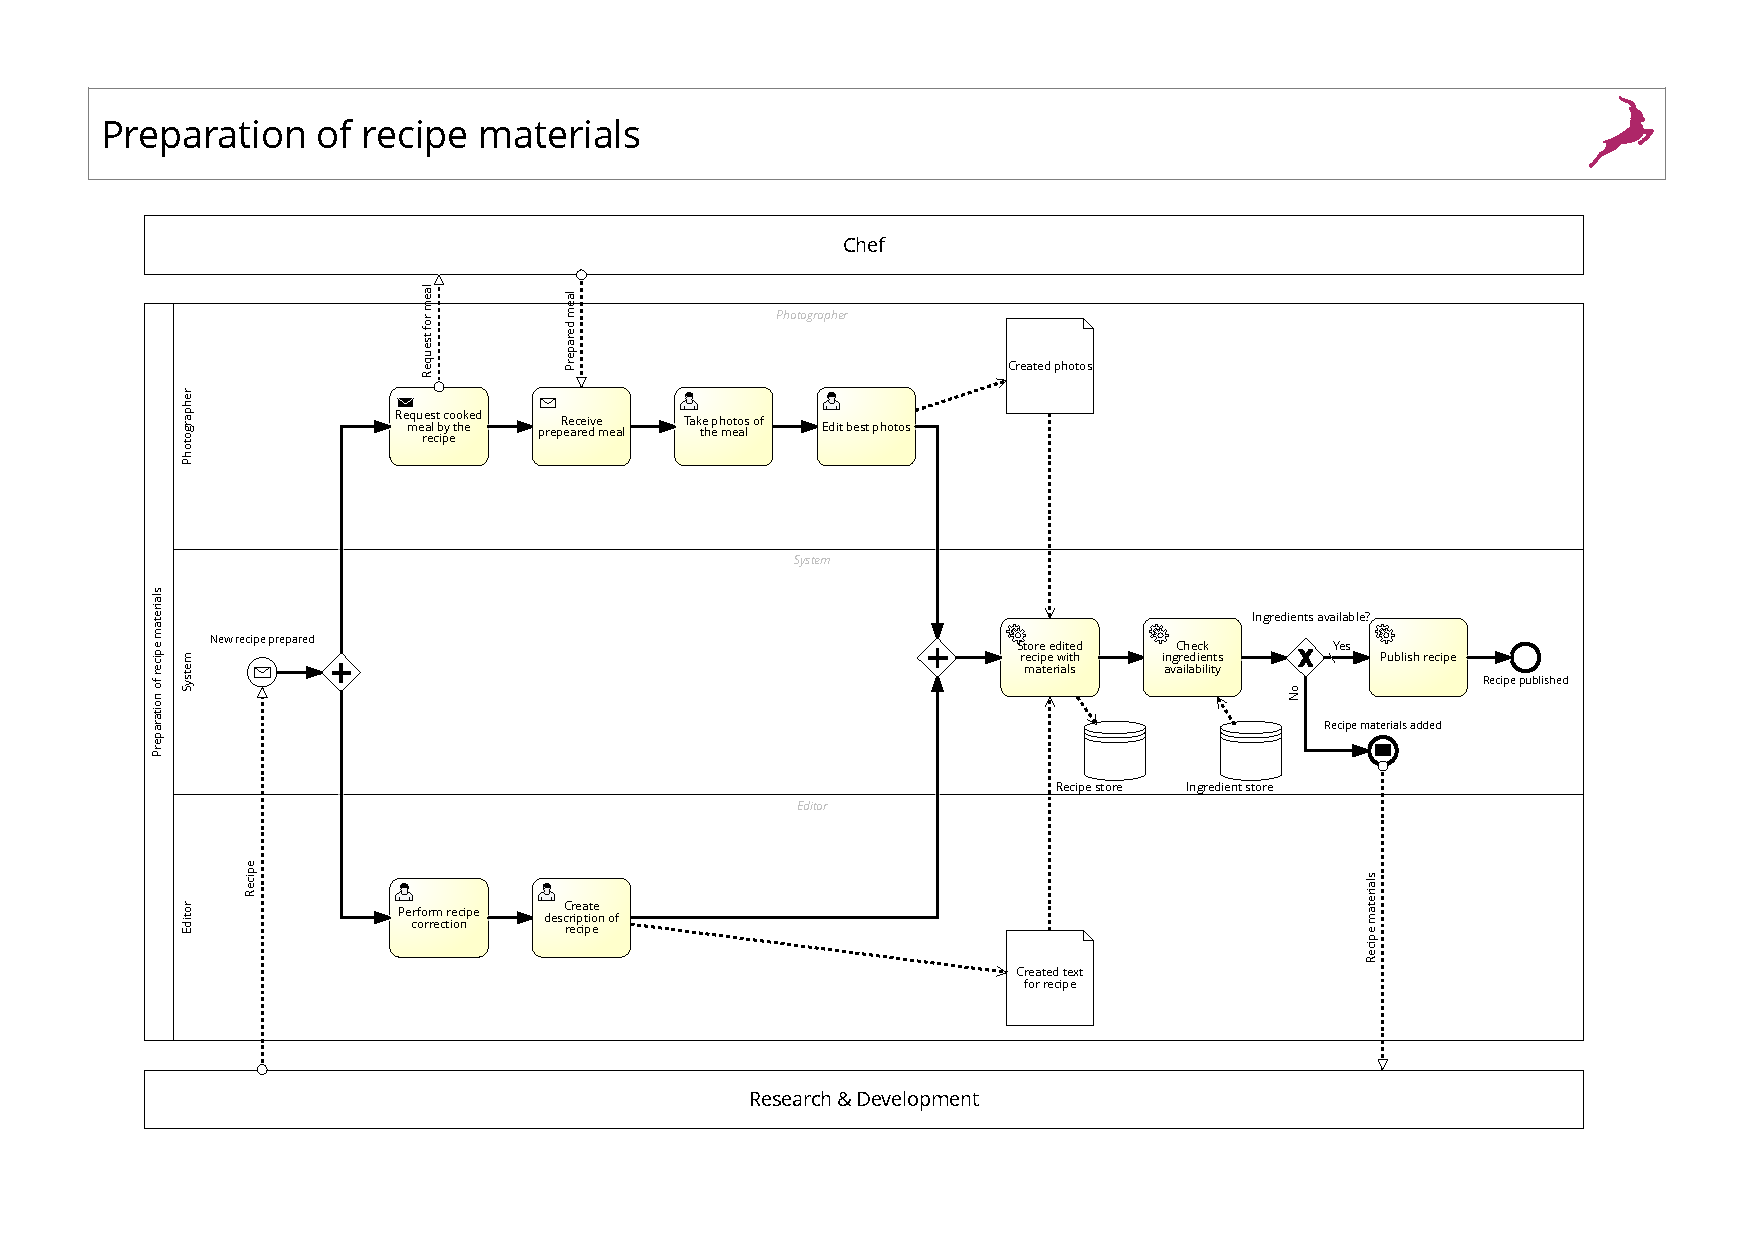
\includepdf[landscape=true]{Preparation of recipe materials.pdf}

%%%%%%%%%%%%%%%%%%%%%%%%%%%%%%%%%%%%%%%%%%%%%%%%%%

\subsection{Process "Find suppliers within a particular distribution center location"}

\paragraph{Description}

This process is situated after manager of distribution center requests for searching suppliers. It is needed to look at which ingredients are requested for recipes. Then some worker has to check warehouse of distribution center which ingredients are missing a ask system to find suppliers for them. System will find supplier by using external searching module. If its response is too long then it's not working and we can't find any suppliers. Otherwise list of suitable suppliers will be received. The worker will have to negotiate with suppliers and then decide if negotiated prices are good for the company. After that manager is informed about negotiated suppliers if there are some. Otherwise he will be informed about reasons of failure.

\paragraph{Indicators}

\begin{itemize}
    \item \textbf{KPI}: Negotiated offers from suppliers. (At least 1 per day)
    \item \textbf{KRI}: Total successfully closed agreements with negotiated suppliers per month. (At least 10 agreements)
\end{itemize}

\paragraph{Roles}

\begin{itemize}
    \item \textbf{Warehouse Worker} - Looks after warehouse and items in it, says what is missing to system, negotiates with suppliers and decides which prices are acceptable.
    \item \textbf{System} - Works with storage, checks for ingredients, communicates with searching module, generates report for manager.
    \item \textbf{Distribution Center Manager} - Starts process by request for searching of suppliers and gets notified about result.
    \item \textbf{IT department} - Gets notified if there are issues with store.
    \item \textbf{Searching module} - Searches for nearby suppliers based on criteria formulated by Warehouse Worker, provides suppliers suiting criteria to system.
    \item \textbf{Supplier} - Negotiates with Warehouse Worker about prices of ingredients.
    
\end{itemize}

\paragraph{Data objects}

\begin{itemize}
    \item \textbf{Store} - Storage for ingredients and recipes.
    \item \textbf{Supplier store} - Storage for suppliers who negotiated with Warehouse Worker.
\end{itemize}

\newpage

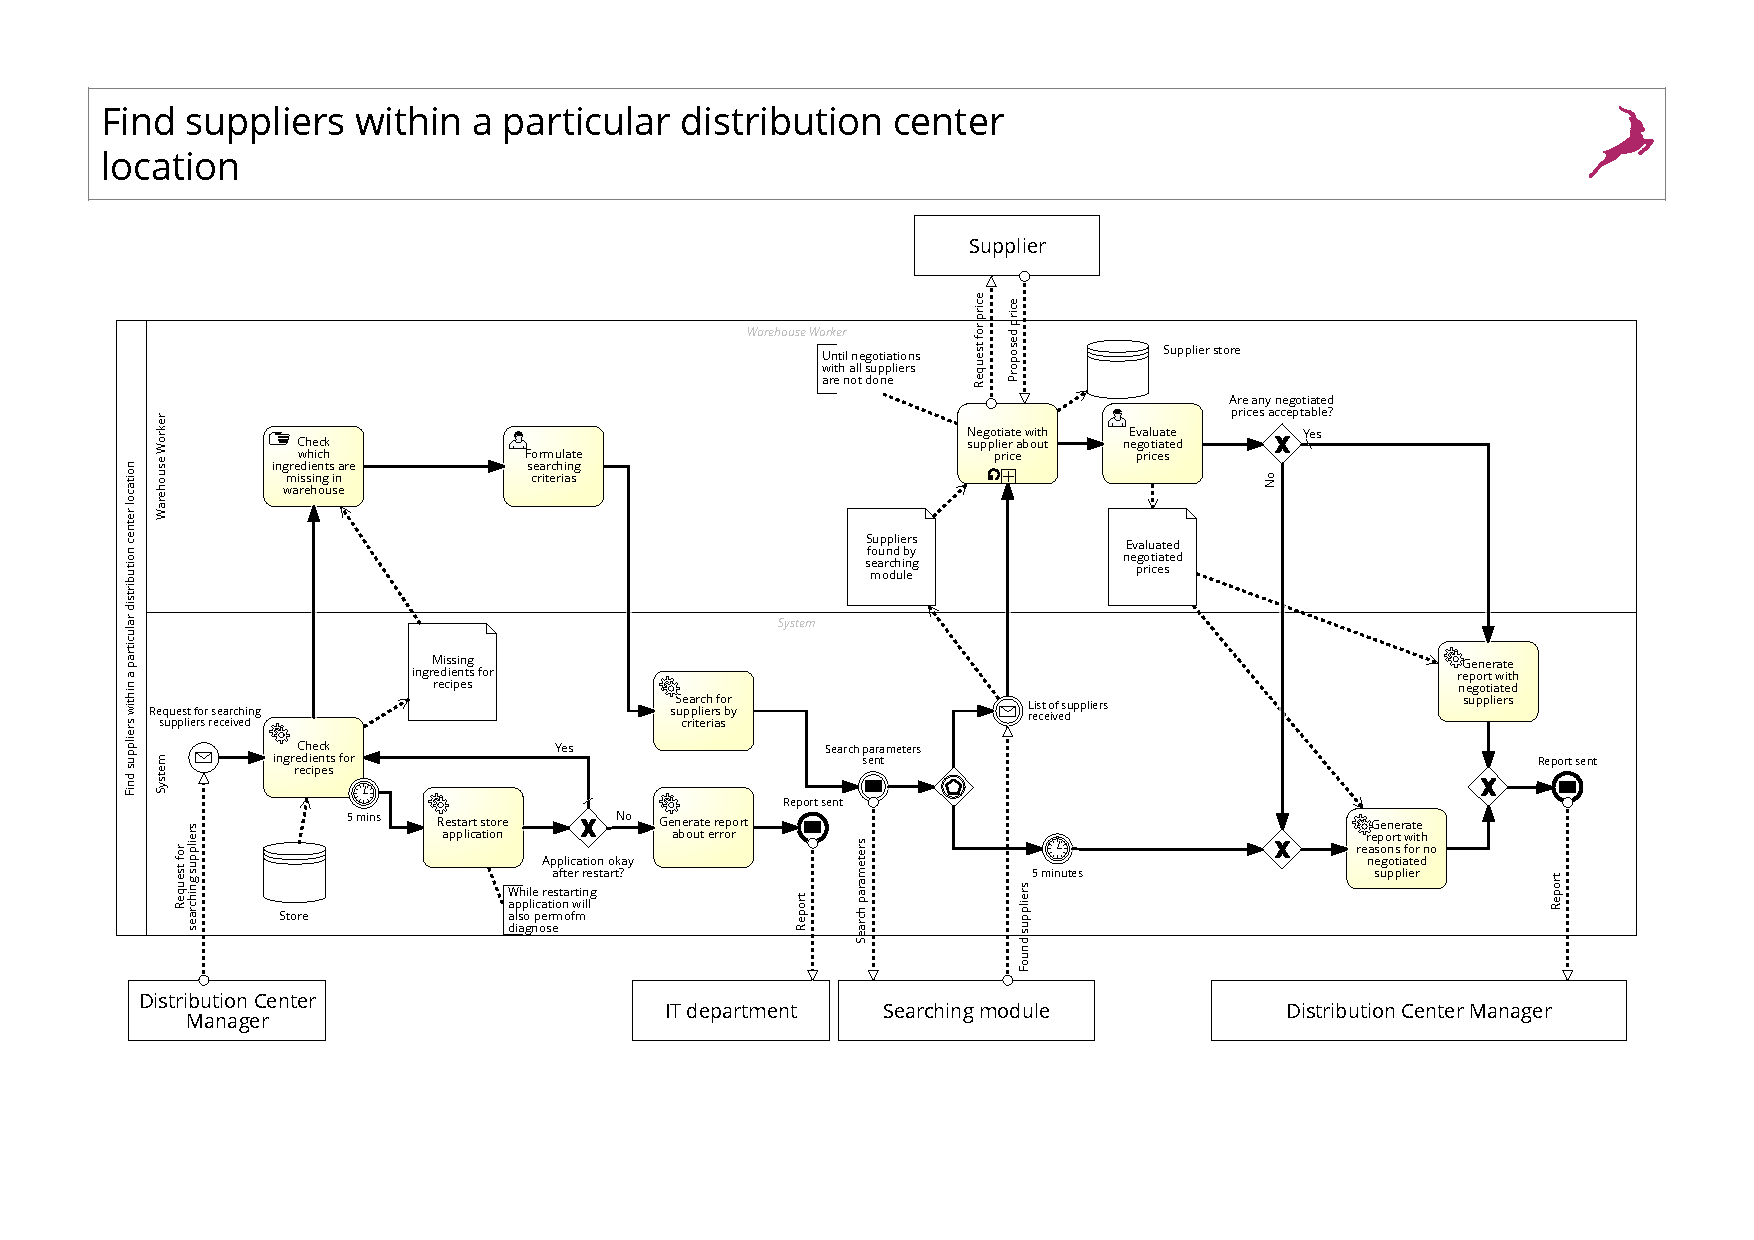
\includepdf[landscape=true]{Find suppliers within a particular distribution center location.pdf}

%%%%%%%%%%%%%%%%%%%%%%%%%%%%%%%%%%%%%%%%%%%%%%%%%%

\subsection{Process "Find experienced chef"}

\paragraph{Description}

Process starts with request for new chef from research and development (RD) department. Management writes offer of working conditions and requirements for chef's experience and education. Human resources (HR) department creates and publish job advert. If no one responds within one week, management adjust job requirements as necessary and HR department updates and publish job advert. When some chef sends job application to HR department, HR department checks if requirements are met. Then HR department sends an assignment to write recipes from prescribed ingredients to chef. If chef does not respond within 3 days, his application is rejected. If chef sends recipes, HR department checks if requirements are met and pass recipes to management. Management checks quality of recipes. If quality of recipes is sufficient, management set salary limit for chef. Then HR department negotiate salary with chef. Chef is accepted if he accepts offered salary within the limit. RD department is informed.

\paragraph{Indicators}

\begin{itemize}
    \item \textbf{KPI}: Number of applications for chef position per day. (At least 1 application)
    \item \textbf{KRI}: Total number of accepted recipes per month. (At least 6 recipes)
\end{itemize}

\paragraph{Roles}

\begin{itemize}
    \item \textbf{CEO} - Writes and updates job requirements. Checks quality of recipes and sets limit on the salary offer.
    \item \textbf{Human Resources Department} - Creates, updates and publish job advert. Checks job application from chef. Sends assignment to chef and verify compliance. Negotiate salary with chef.
    \item \textbf{Research \& Development Department} - Requests new chef.
    \item \textbf{Chef} - Applies for job and creates recipes from prescribed ingredients.
\end{itemize}

\paragraph{Data objects}

\begin{itemize}
    \item \textbf{Job offer and requirements} - Education and experience requirements for a new cook.
    \item \textbf{New job offer and requirements} - Updated education and experience requirements for a new cook.
    \item \textbf{Recipes} - Verified recipes.
\end{itemize}

\newpage

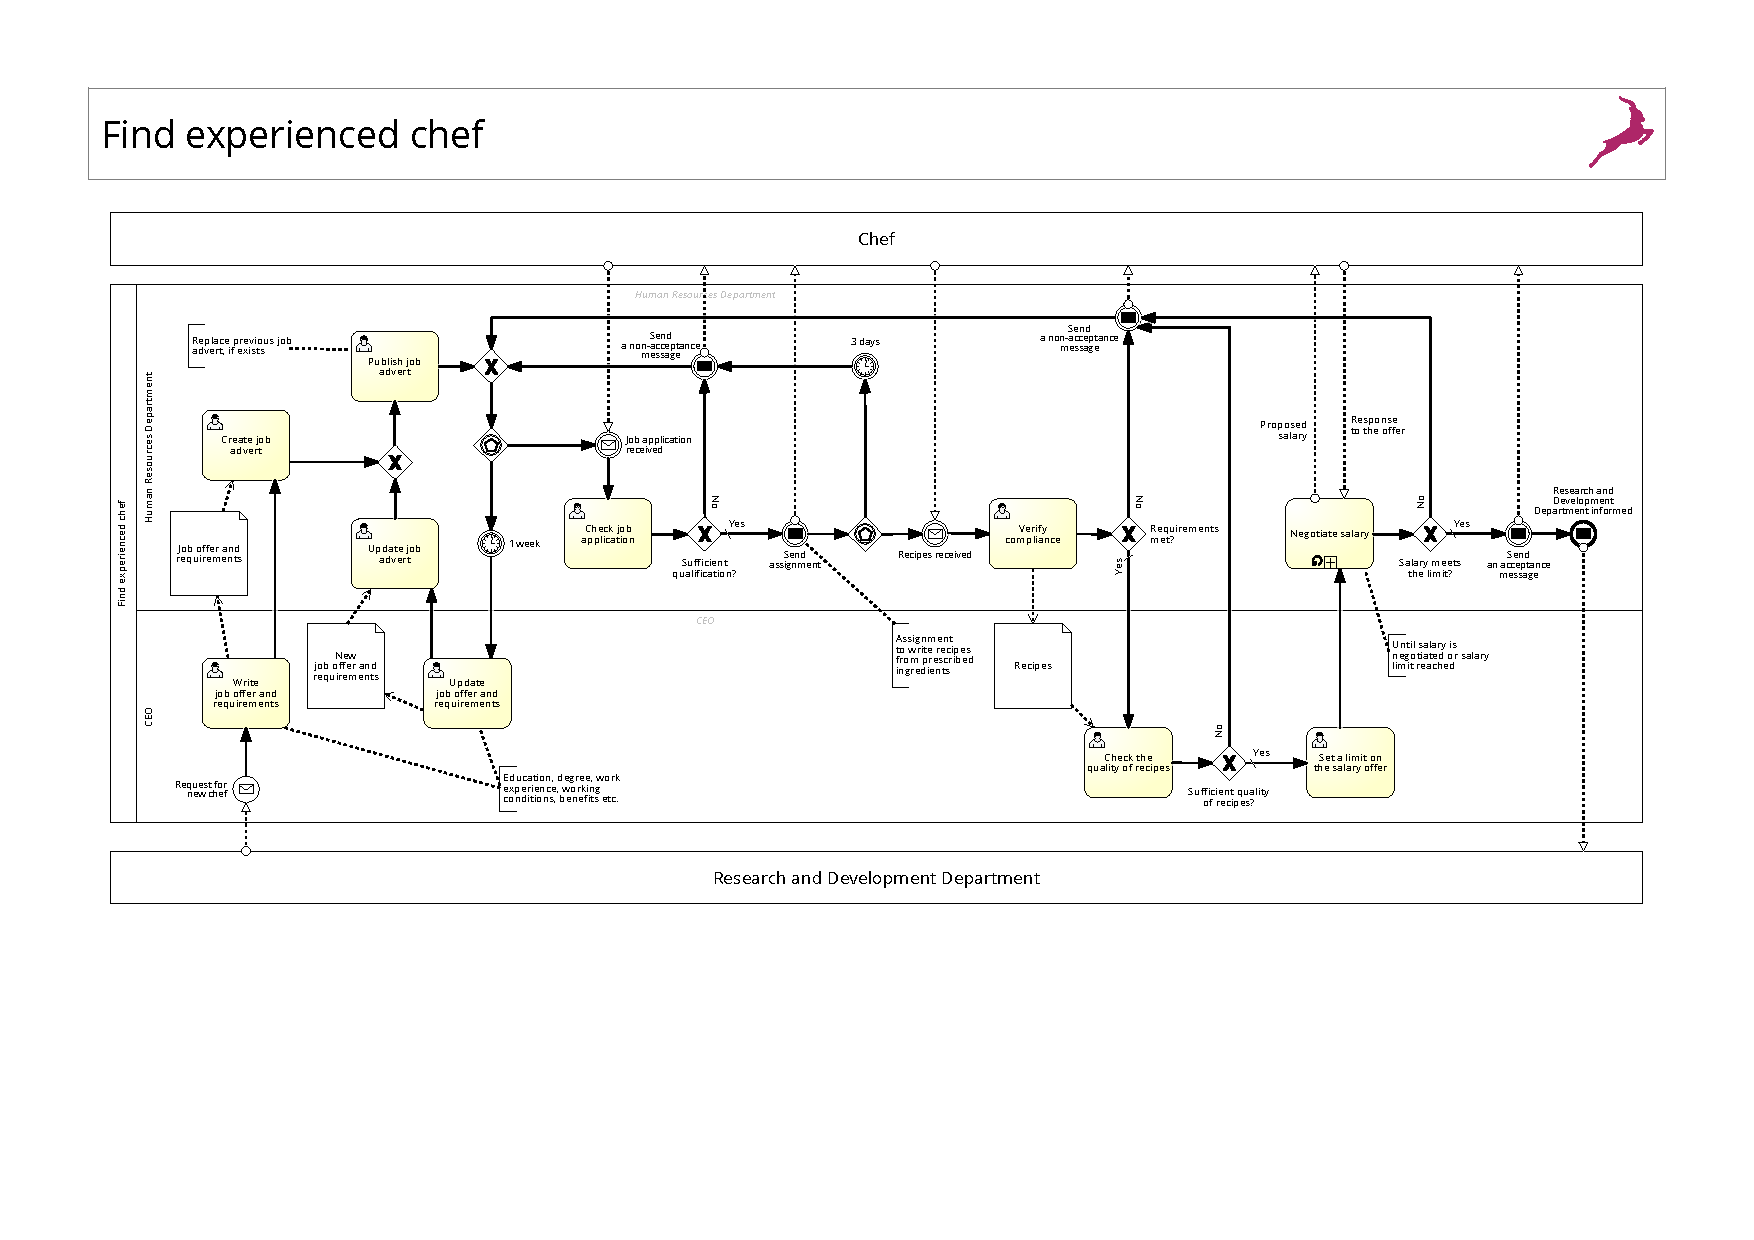
\includepdf[landscape=true]{Find experienced chef.pdf}

%%%%%%%%%%%%%%%%%%%%%%%%%%%%%%%%%%%%%%%%%%%%%%%%%%

\subsection{Process "Route planning"}

\paragraph{Description}

Process is situated after choosing and approval of new distribution center by CEO. At first logistics manager has to decide if enough drivers are available for new distribution center. Then he has to plan routes for distribution center. After planning of routes, he needs to assign routes and drivers to distribution centers. CEO has to approve new changes of distribution centers, drivers and routes. New data are saved and drivers are notified about their assigned distribution centers and about routes assigned to these distribution centers.

\paragraph{Indicators}

\begin{itemize}
    \item \textbf{KPI}: Daily number of orders delivered on time. (At least 90 \% orders)
    \item \textbf{KRI}: Total number of orders delivered on time per month. (At least 95 \% orders)
\end{itemize}

\paragraph{Roles}

\begin{itemize}
    \item \textbf{CEO} - Checks the distribution of drivers and routes.
    \item \textbf{System} - Works with storage, sends assignment to drivers
    \item \textbf{Logistics Manager} - Plans routes, assigns routes and drivers to distribution centers, requests new drivers.
    \item \textbf{Human Resources Department} - Gets new drivers if needed.
    \item \textbf{Driver} - Receives info about assigned routes and distribution center.
\end{itemize}

\paragraph{Data objects}

\begin{itemize}
    \item \textbf{Store} - Storage for distribution centers with assigned routes and drivers.
    \item \textbf{Distribution centers with drivers and routes} - All distribution centers with assigned routes and drivers before planning.
    \item \textbf{Distribution centers with assigned routes and drivers} - All distribution centers with assigned routes and drivers after planning.
\end{itemize}

\newpage

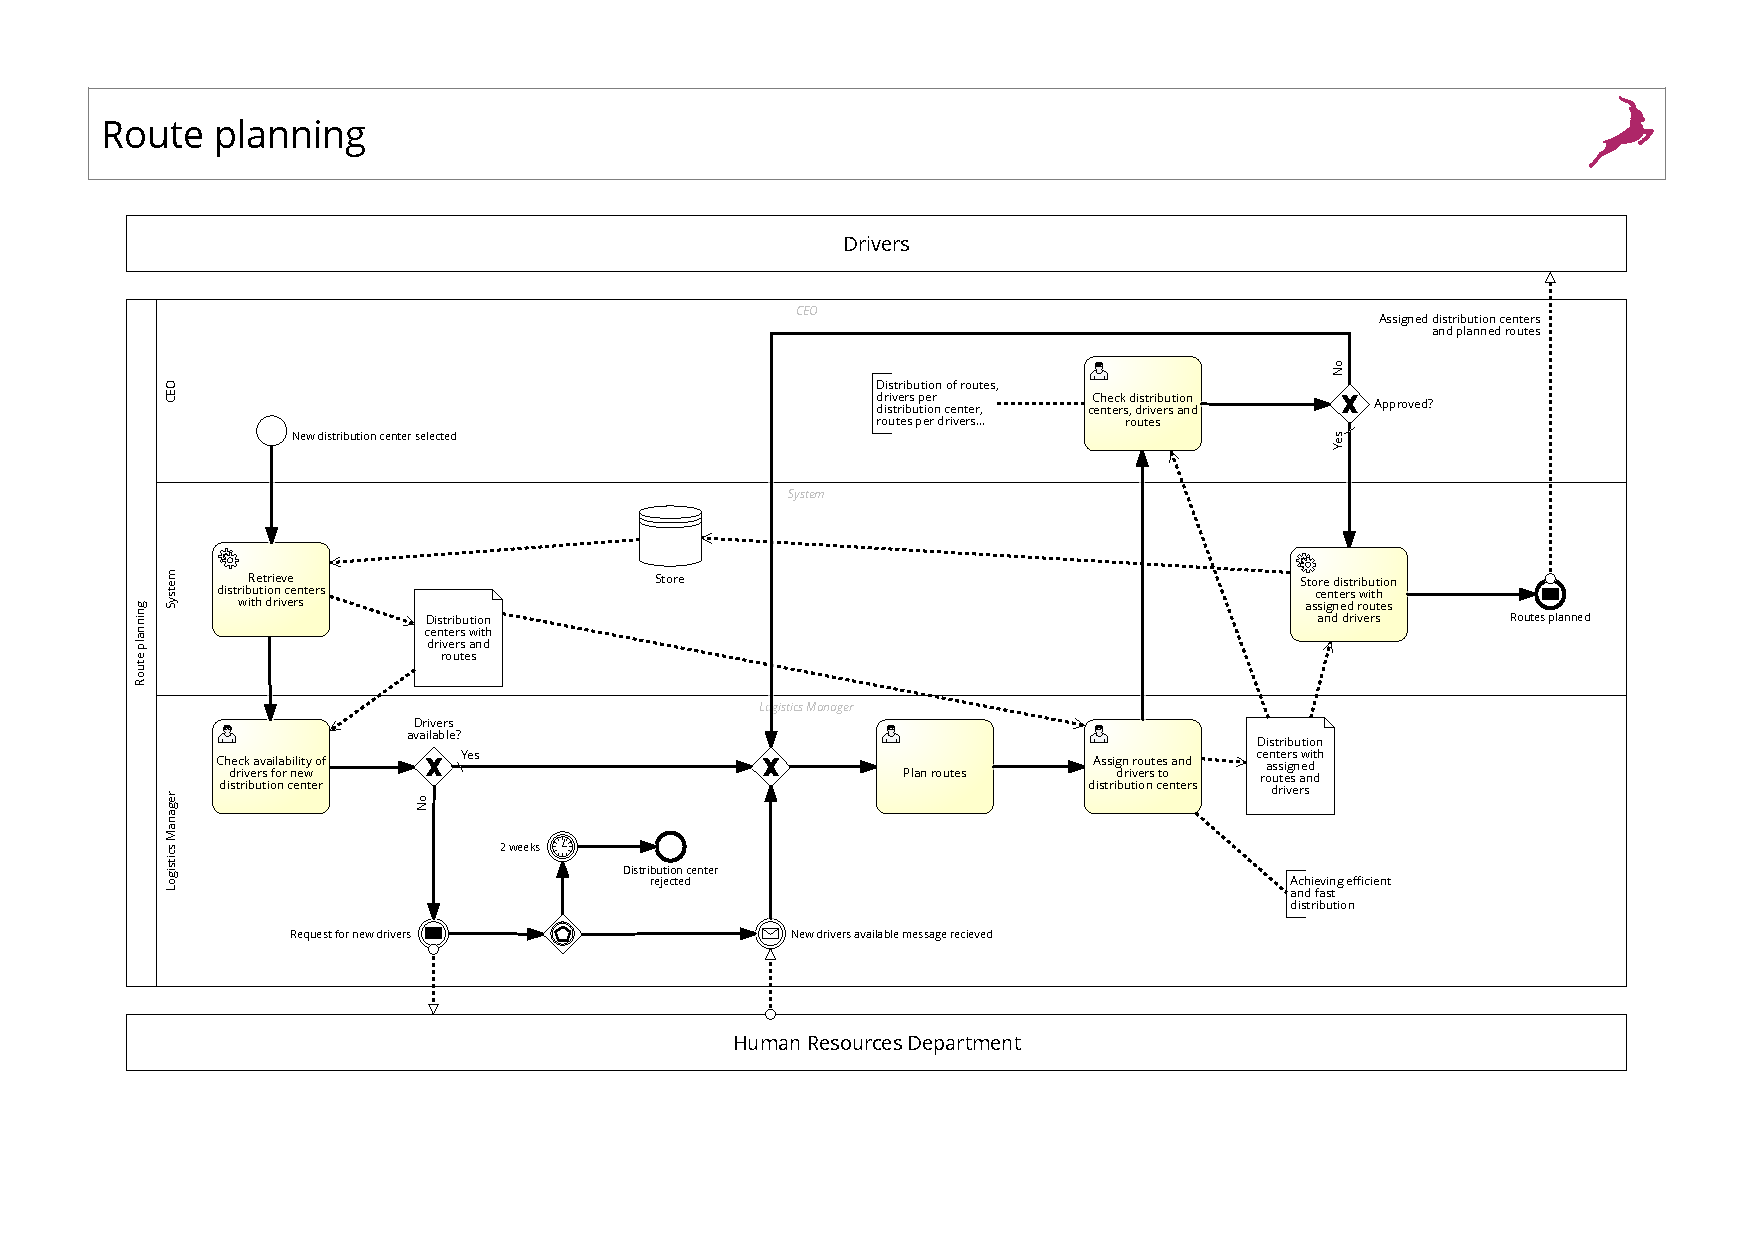
\includepdf[landscape=true]{Route planning.pdf}

%%%%%%%%%%%%%%%%%%%%%%%%%%%%%%%%%%%%%%%%%%%%%%%%%%

\subsection{Process "Create statistical report for CEO"}

\paragraph{Description}

CEO can request statistical report from all managers about orders, suppliers, supplies, distribution centers and drivers. System provides statistical data for all managers and they prepare report. System processes all these reports and unify them into one report for CEO. Report is sent to CEO.

\paragraph{Indicators}

\begin{itemize}
    \item \textbf{KPI}: Number of days without reports about orders and other aspects. (At most 2 days)
    \item \textbf{KRI}: Ratio of positive reports from managers per year. (At least 90 \% positive reports)
\end{itemize}

\paragraph{Roles}

\begin{itemize}
    \item \textbf{CEO} - Requests and receives report.
    \item \textbf{System} - Retrieves statistical data for managers and processes reports.
    \item \textbf{Logistics Manager} - Creates report.
    \item \textbf{Distribution Center Manager} - Creates report.
    \item \textbf{Procurement Officer} - Creates report.
    \item \textbf{Order Manager} - Creates report.
\end{itemize}

\paragraph{Data objects}

\begin{itemize}
    \item \textbf{Store} - Storage for statistical data.
    \item \textbf{Statistical data} - All statistical data over a period of time.
    \item \textbf{Report} - Created report by manager.
\end{itemize}

\newpage

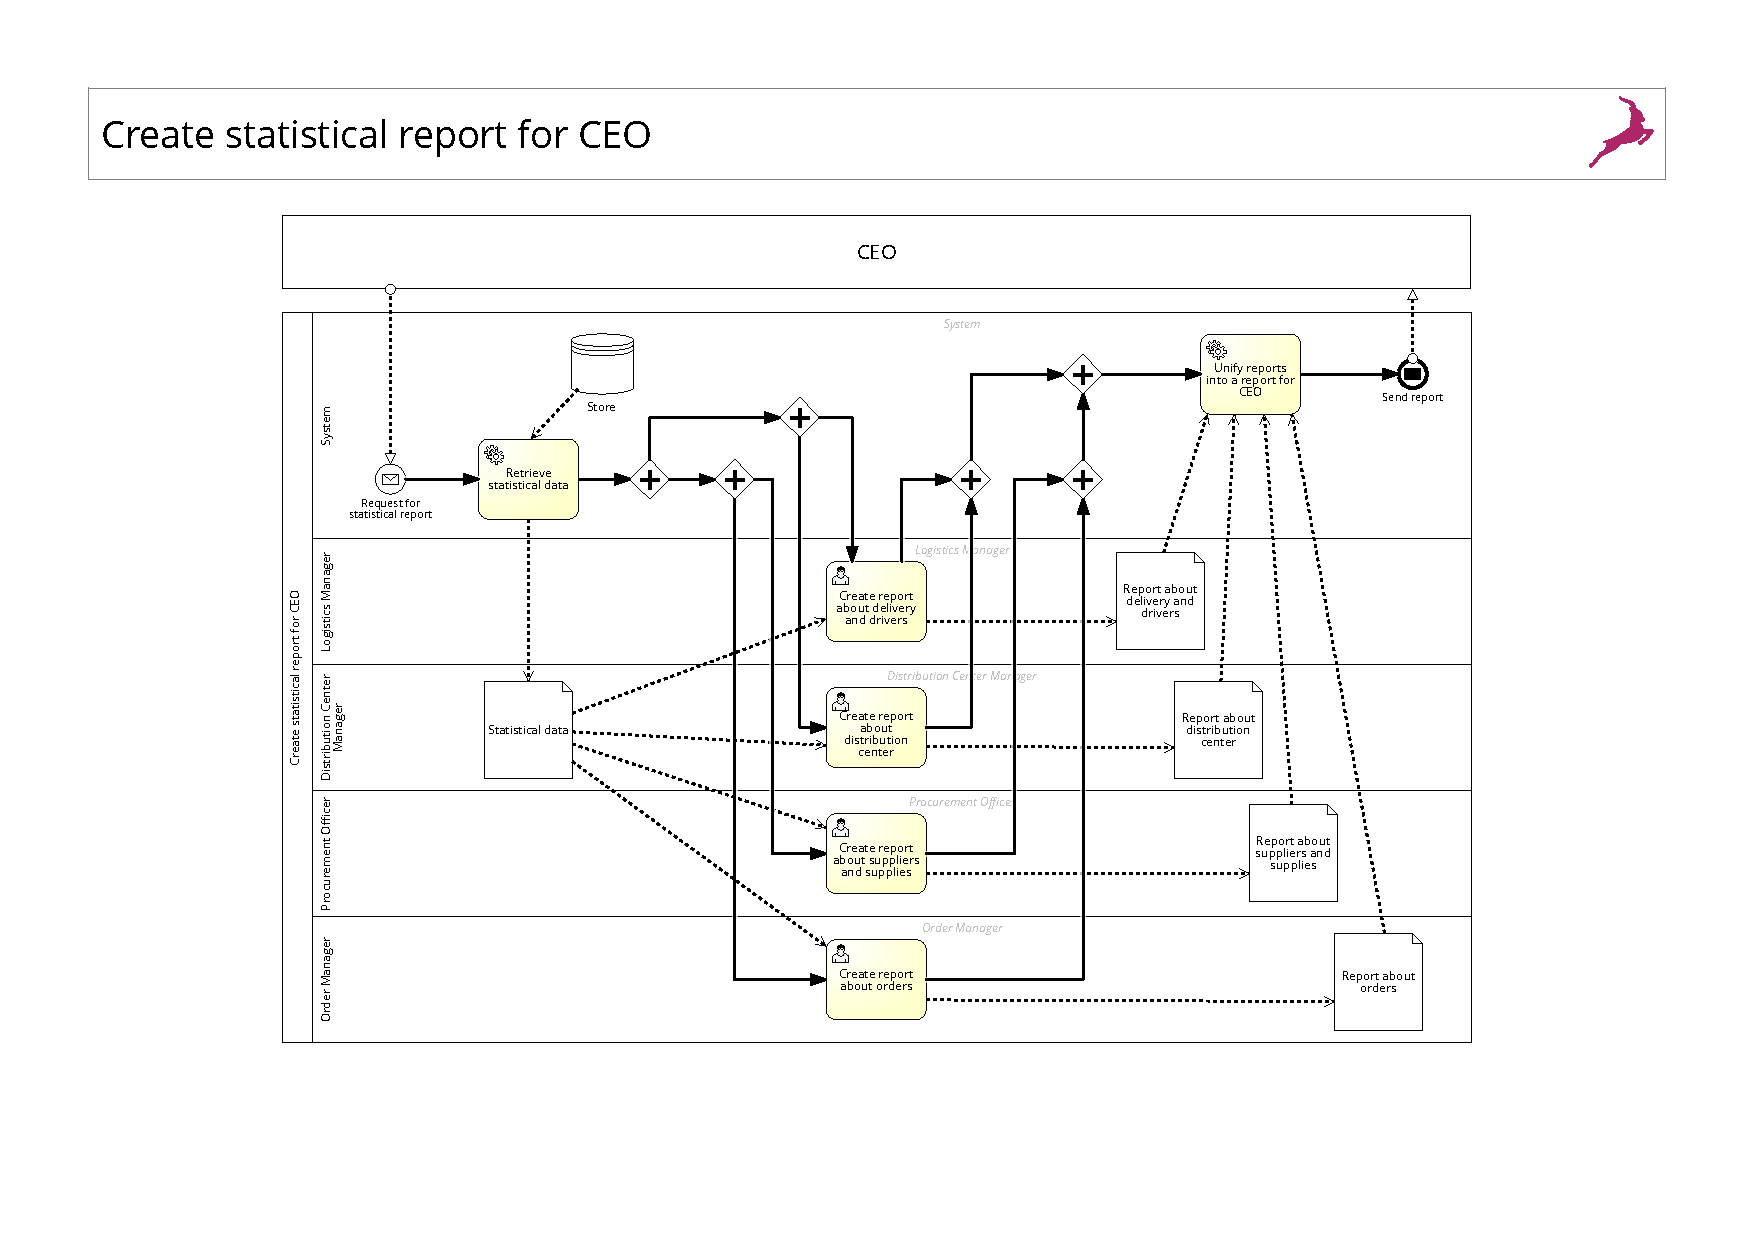
\includepdf[landscape=true]{Create statistical report for CEO.pdf}

%%%%%%%%%%%%%%%%%%%%%%%%%%%%%%%%%%%%%%%%%%%%%%%%%%

\subsection{Process "Create new recipe"}

\paragraph{Description}
The process is expected to run several times at the beginning of every week in order to produce new recipes. The created recipe serves as a base for a following process, \emph{Preparation of recipe materials}.

\medskip

Initially, the \textbf{marketing department} examines user feedback and creates a trend analysis from current and upcoming trends. Afterwards, the \textbf{R\&D department} proposes recipe ideas until a suitable candidate is agreed upon. The chosen idea is handed over to an experienced \textbf{chef} who composes a recipe prototype. The prototype is saved for future use, regardless of the eventual approval or abandonment of the recipe. Feasibility check, consisting of price estimation and recipe execution testing, is performed. Assuming the feasibility result is positive, the recipe is approved. In the scenario of negative result, an abandonment report is generated. In the end, the \textbf{information system} is notified with the approved recipe or abandonment report.

\paragraph{Indicators}

\begin{itemize}
    \item \textbf{KPI}: Time to develop a recipe. (Less than a week)
    \item \textbf{KRI}: Total number of developed recipes per month. (At least 6 recipes)
\end{itemize}

\paragraph{Roles}

\begin{itemize}
    \item \textbf{Marketing} - Performs trend analysis and retrieves user feedback.
    \item \textbf{Research \& Development} - Comes up with recipe ideas, performs recipe feasibility testing, approves recipes, rejects recipes.
    \item \textbf{Chef} - Supplies recipe prototype from provided recipe ideas.
    \item \textbf{System} - Receives information whether the recipe was approved or rejected.
\end{itemize}

\paragraph{Data objects}

\begin{itemize}
    \item \textbf{Recipe store} - All recipes (approves or rejected) are stored for future reference, evaluation or reusing purposes.
    \item \textbf{User feedback} - User feedback and wishes towards recipes and food content are considered during proposing of new recipe ideas. Supplied by marketing department.
    \item \textbf{Recipe store} - Current trends and estimation of future trends are considered during proposing of new recipe ideas. Supplied by marketing department.
\end{itemize}

\newpage

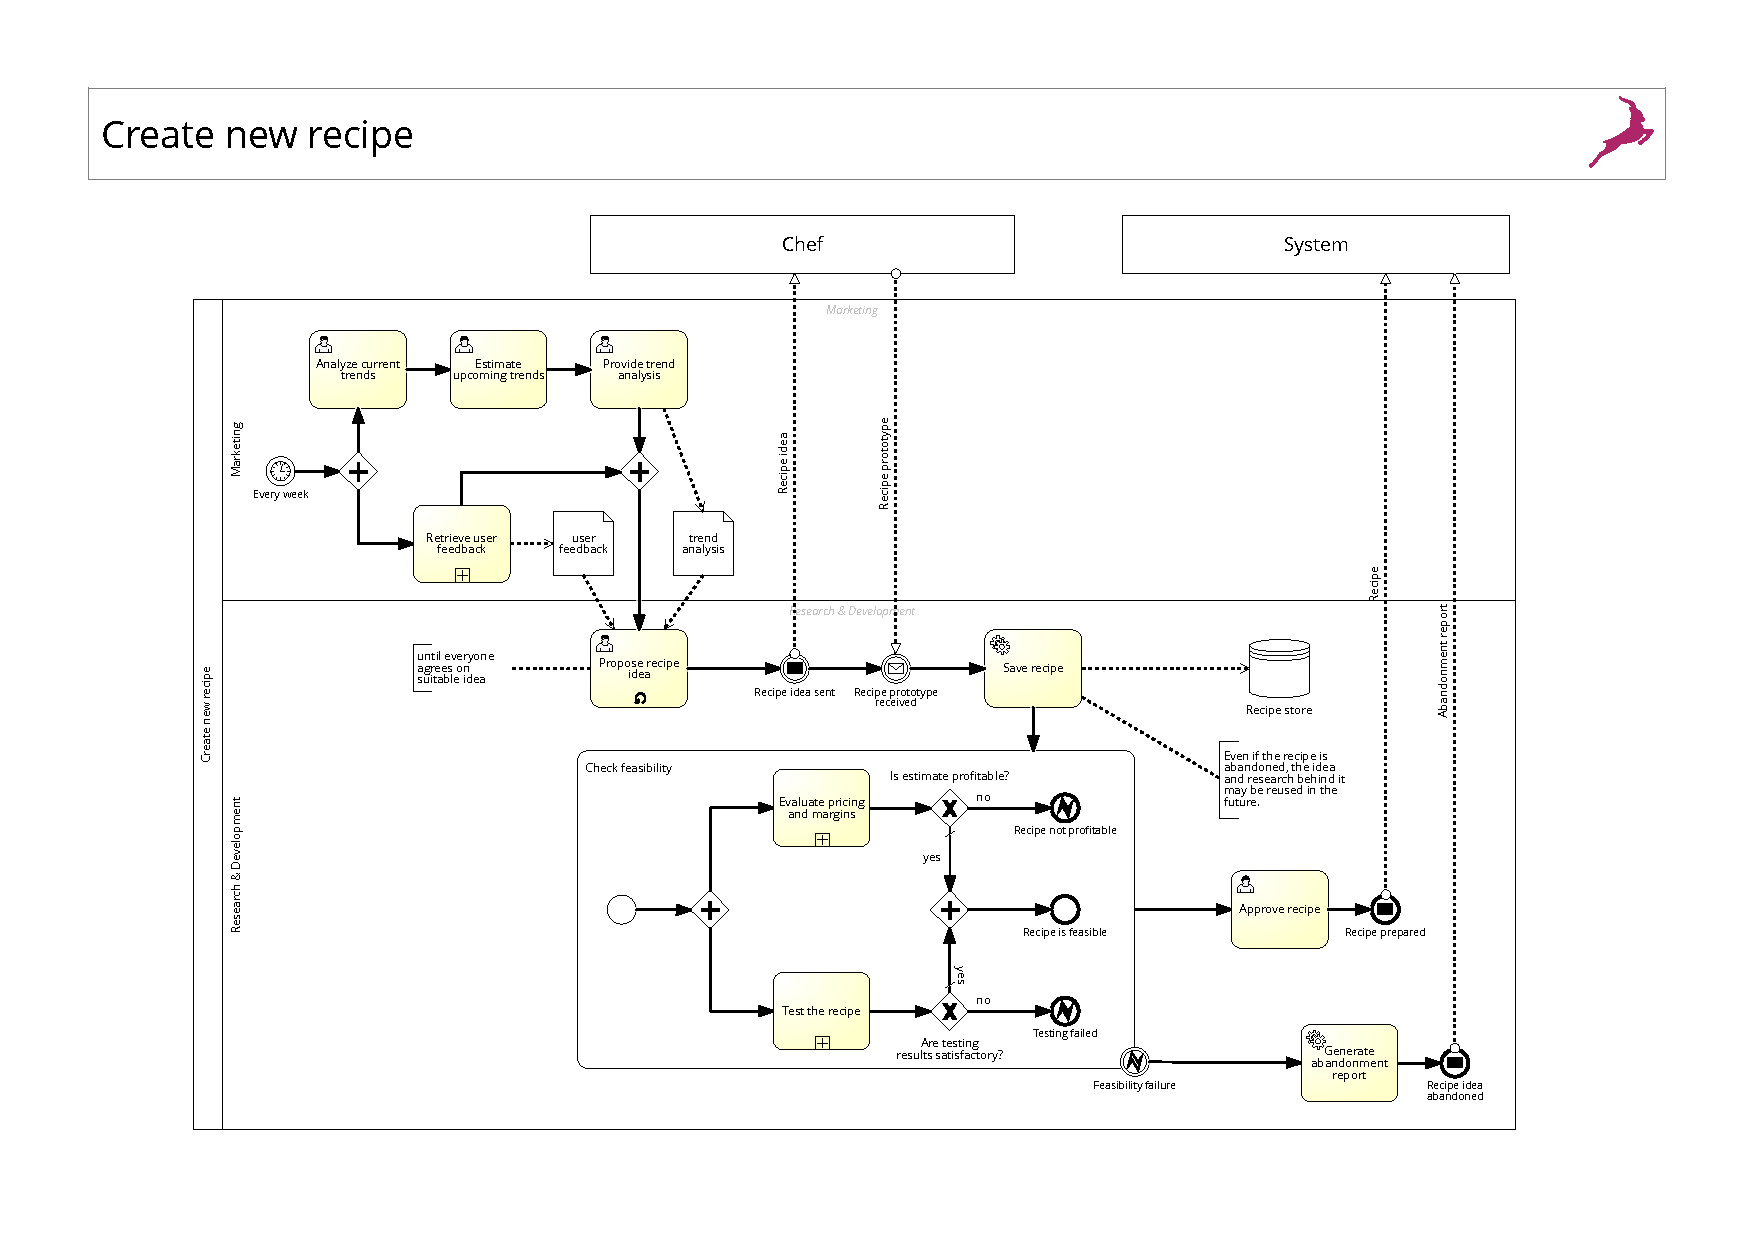
\includepdf[landscape=true]{create_new_recipe.pdf}

%%%%%%%%%%%%%%%%%%%%%%%%%%%%%%%%%%%%%%%%%%%%%%%%%%

\subsection{Process "Customer support"}

\paragraph{Description}
Customer support handles and resolves complaints and problems users encounter. The communication and notification may be in form of e-mail exchange, chat messaging or voice/phone call. Initially, system acknowledges new ticket, creates an issue and checks whether the ticket is not disingenuous. Afterwards, support worker reviews the problem, communicates with the customer, evaluates possible solutions and if possible handles the issue and informs the customer about the result of the issue. Support manager may step in if support worker requires help or any form of advice. Furthermore, in cases where higher authority is required, support manager may take the handling of the issue on himself/herself. The resolution process may find no feasible solution to the problem. In such case, additional attention to the reasoning and final response has to be provided.

\paragraph{Indicators}

\begin{itemize}
    \item \textbf{KPI}: Number of issues per day. (Maximum 100 reports of issues)
    \item \textbf{KRI}: Ratio of solved issues per month. (At least 70 \% solved issues)
\end{itemize}

\paragraph{Roles}

\begin{itemize}
    \item \textbf{Customer} - Submits a ticket, communicates his/her problem, receives notifications.
    \item \textbf{System} - Receives tickets, registers issues, performs automatic assessments (eliminates invalid tickets etc.).
    \item \textbf{Support Worker} - Reviews customer's problem, communicates with customers, finds a solution and handles problem.
    \item \textbf{Support Manager} - Gives advice to support worker and handles the issue if circumstances require it (support worker for whatever reason isn't capable of doing it).
\end{itemize}

\paragraph{Data objects}

\begin{itemize}
    \item \textbf{Issue store} - All customer complaints and issues are stored in the system.
\end{itemize}

\newpage

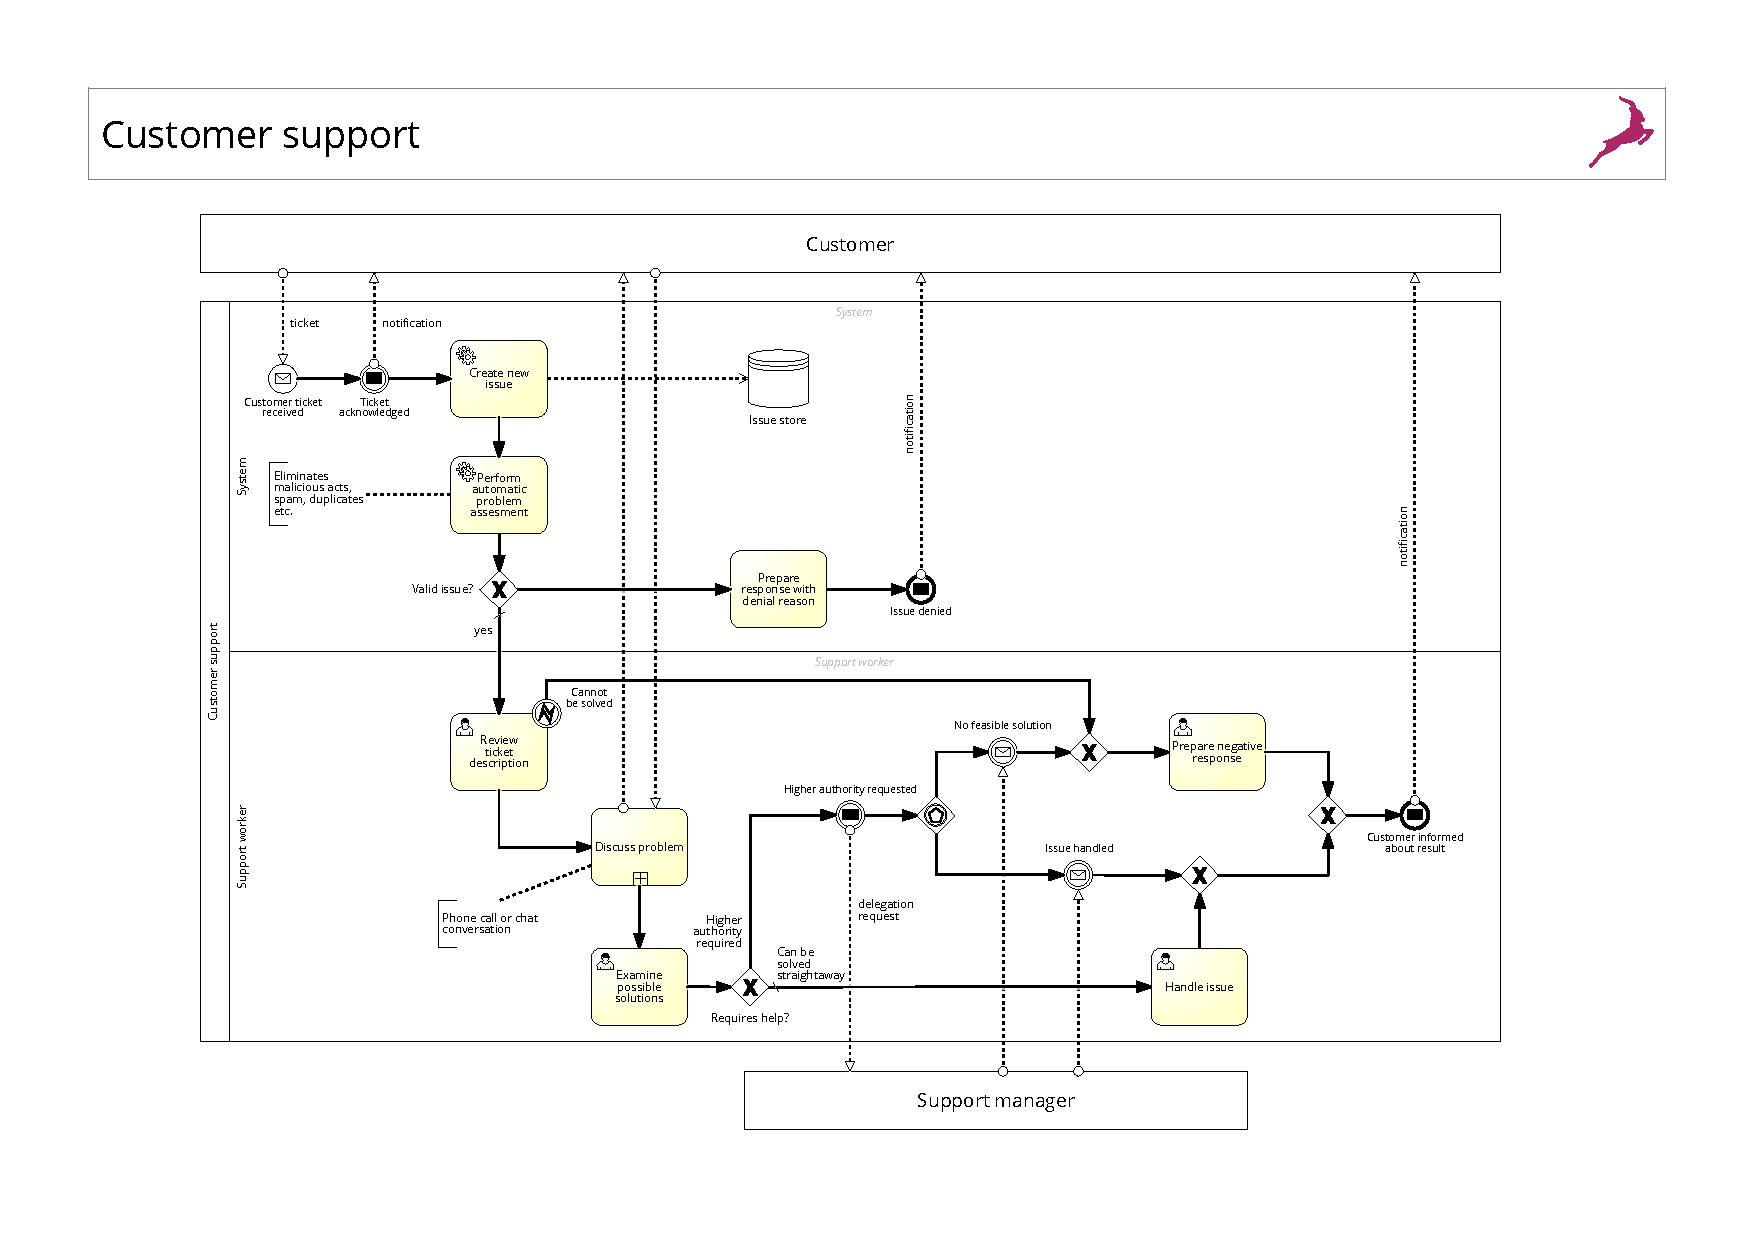
\includepdf[landscape=true]{customer_support.pdf}

%%%%%%%%%%%%%%%%%%%%%%%%%%%%%%%%%%%%%%%%%%%%%%%%%%

\subsection{Process "Order processing"}

\paragraph{Description}
Our company provides high quality recipes with on demand high quality ingredients for people to cook themselves in the form of fast and convenient FoodPacks. When new order is received the initial processing must last less then two hours (including receiving payment) due to high fluctuations in warehouse or ad-hoc ingredient orders. When resources for a set of orders have been acquired and prepared it is time to pack them in the actual packaging, and prepare them for delivery in proper conditions. The process of packaging is straight forward, however, it can come to a situation when an ingredients is missing. Again, this has to be resolved fast. After all is done someone just need to pick it up.

\paragraph{Indicators}

\begin{itemize}
    \item \textbf{KPI}: Average speed of order fulfillment. (Average 2 days)
    \item \textbf{KRI}: Overall customer satisfaction with delivered goods \& packaging. (At least 90 \% of satisfied customer)
\end{itemize}

\paragraph{Roles}

\begin{itemize}
    \item \textbf{Packaging worker} - Prepares the package ensuring nothing will be left out.
    \item \textbf{Order management officer} - Validates orders and makes sure the order will reach customer's door.
    \item \textbf{System} - Handles orders and order payments.
    \item \textbf{Procurement} - Allocates resources upon request.
    \item \textbf{Customer} - Receives updates.
\end{itemize}

\paragraph{Data objects}

\begin{itemize}
    \item \textbf{List of orders} - List of all orders addressed to a packaging worker that need to be packed.
\end{itemize}

\newpage

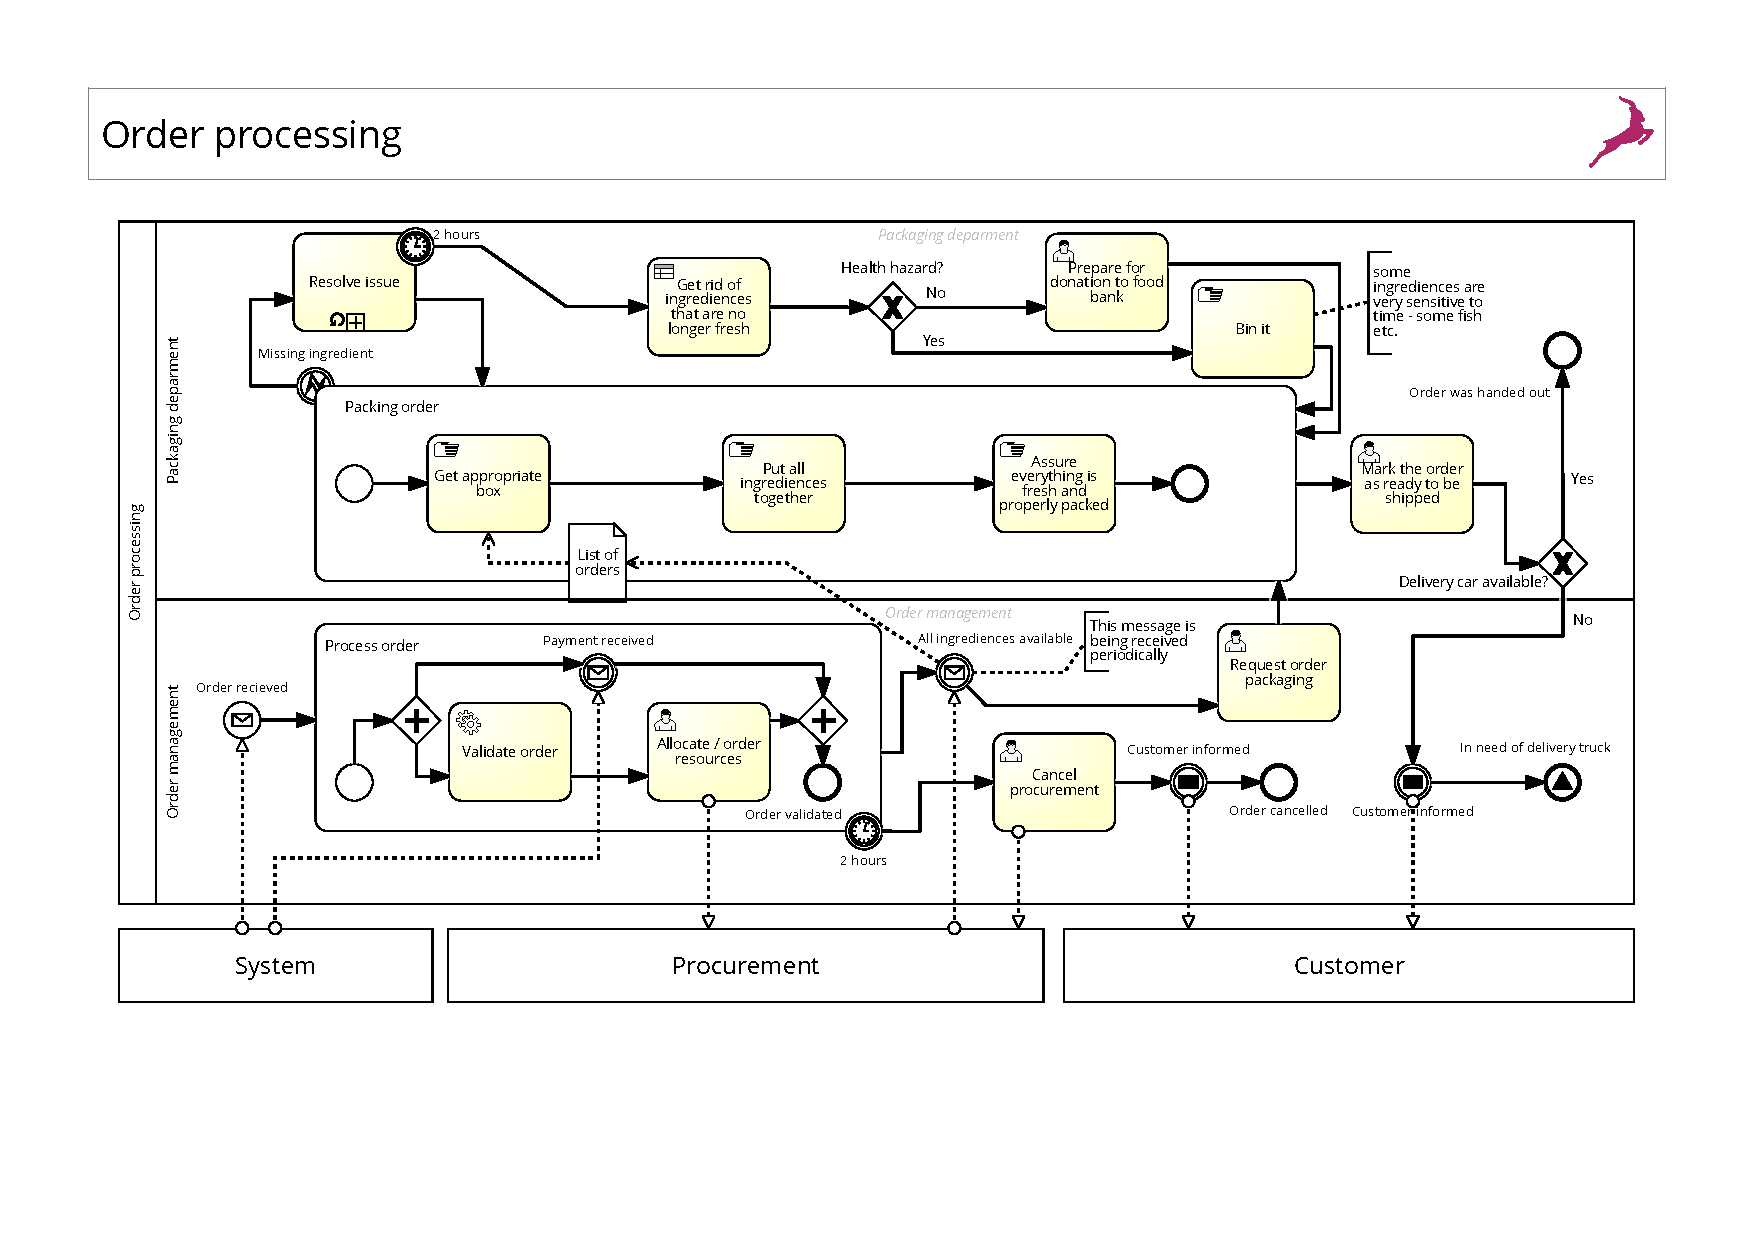
\includepdf[landscape=true]{order_processing.pdf}

%%%%%%%%%%%%%%%%%%%%%%%%%%%%%%%%%%%%%%%%%%%%%%%%%%

\subsection{Process "Create a promotion campaign"}

\paragraph{Description}
Once a product or an idea is developed it has to reach the audience. Every recipe has to be field tested by our most trusted customers that will be specially targeted and offered a free sample in return of a complete feedback. Company standards state that the rate of positive feedback received has to be larger than 80\% in order to launch a public marketing campaign in TV or other media. Our marketing partner provides us with created documentation and materials for the developed idea or product by which it will be then promoted in our systems.

\paragraph{Indicators}

\begin{itemize}
    \item \textbf{KPI}: Website hits per day. (At least 5000 hits)
    \item \textbf{KRI}: Conversion rate in UTM (Urchin Tracking Module) source customers per month. (At least 10 \% conversion rate)
\end{itemize}

\paragraph{Roles}

\begin{itemize}
    \item \textbf{Marketing} - Handles public relations and shares targeted offers.
    \item \textbf{Research \& Development} - Develops new ideas.
    \item \textbf{Customers} - Provide feedback.
    \item \textbf{Public} - Consume information.
    \item \textbf{Marketing company} - A creative marketing company that has long history of creating successful campaigns.
\end{itemize}

\paragraph{Data objects}

\begin{itemize}
    \item \textbf{Recipe store} - Storage for created recipes.
\end{itemize}

\newpage

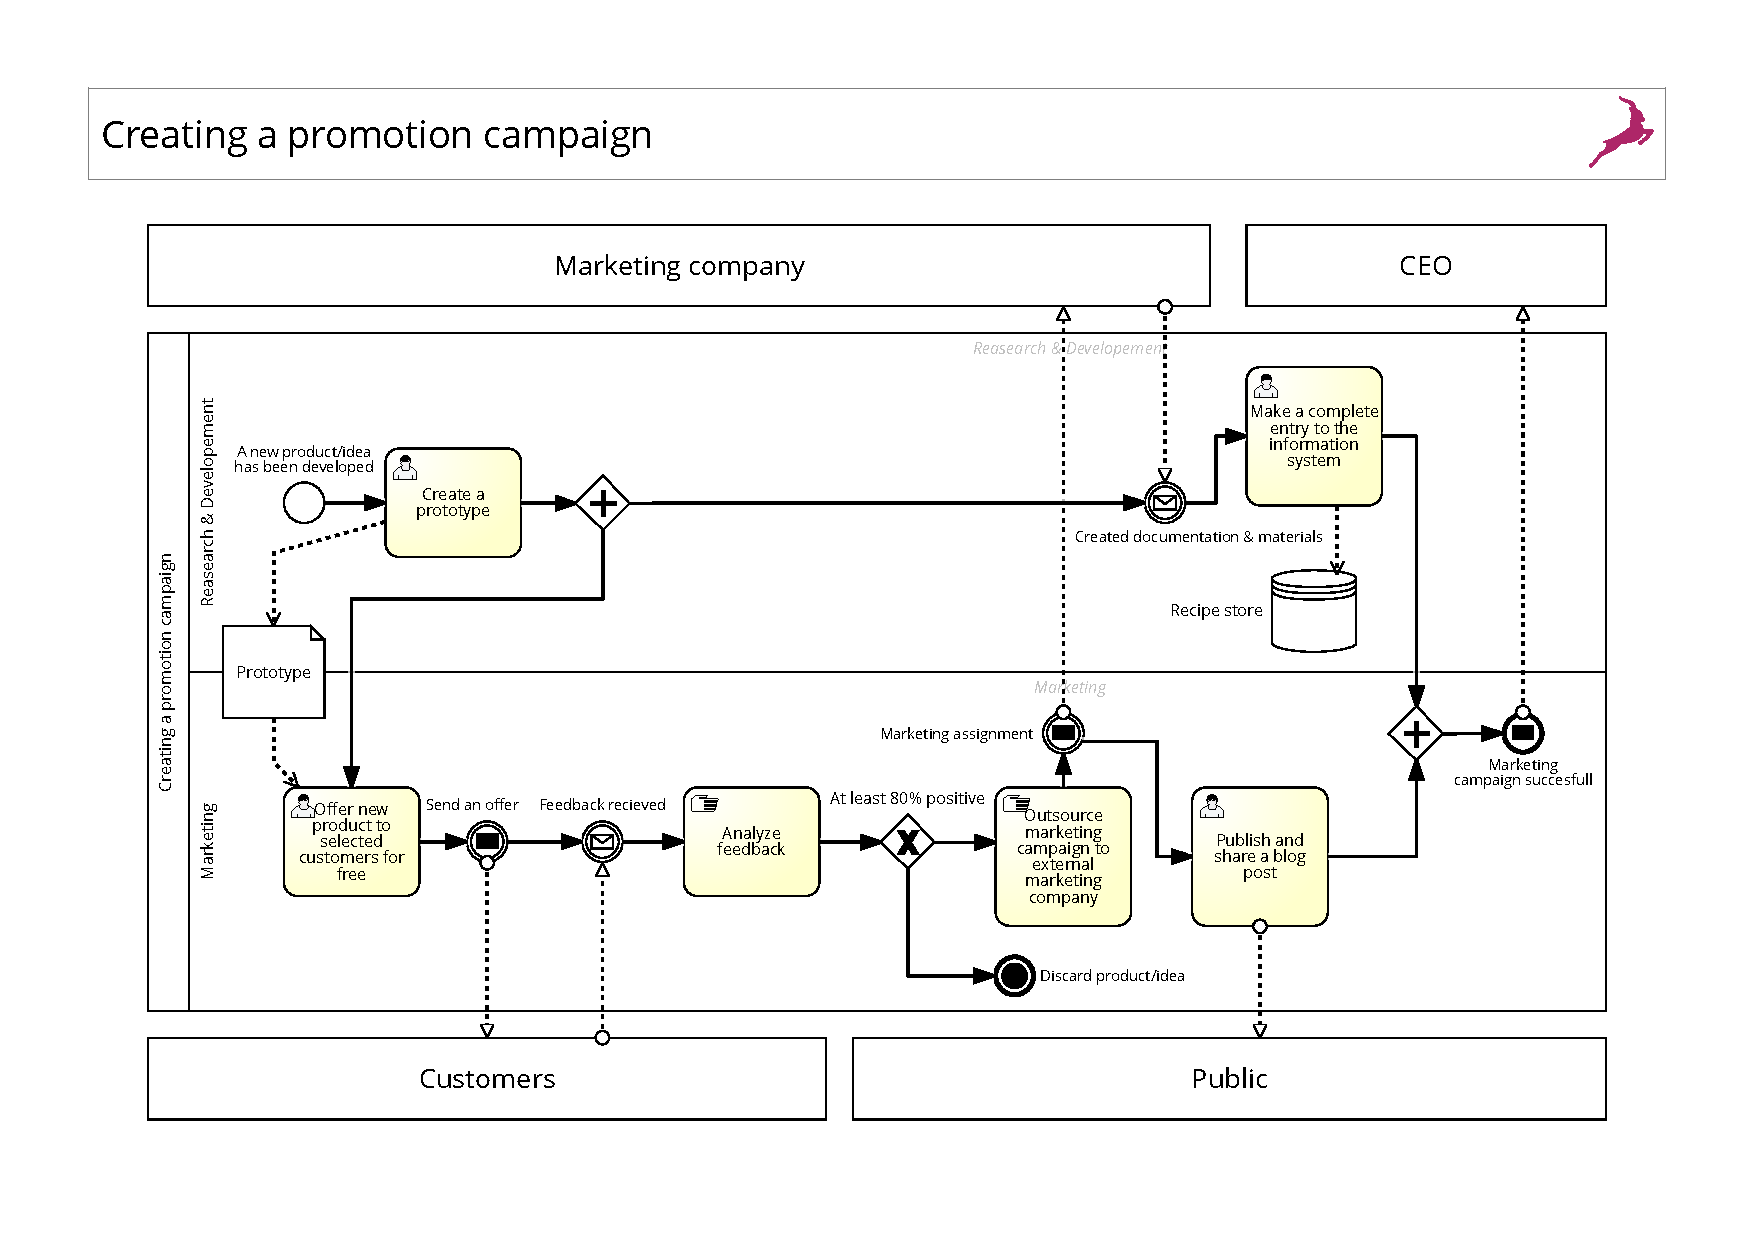
\includepdf[landscape=true]{creating_a_promotion_campaign.pdf}

%%%%%%%%%%%%%%%%%%%%%%%%%%%%%%%%%%%%%%%%%%%%%%%%%%%%%%%%%%%%%%%%%%%%%%%%%%%%%%%%%%%%%%%%%%%%%%%%%%%%%%%%%%%%%

\section{Implementation}

Project can be imported from \url{https://github.com/binczech/PV207-BPM}.

%%%%%%%%%%%%%%%%%%%%%%%%%%%%%%%%%%%%%%%%%%%%%%%%%%

\subsection{Used platform and software}

\begin{itemize}
    \item \textbf{jBPM 7.36.0.Final} - This tool was chosen because it was the only tool that had been presented on lectures. Also there was support provided by teachers for this tool. We chose version 7.36.0.Final because it was the latest version at that time. We also didn't switch to version 7.37.0.Final afterwards because there were many bugs reported by students or other users for this version.\footnote{jBPM 7.36.0.Final can be downloaded from \url{https://download.jboss.org/jbpm/release/7.36.0.Final/jbpm-server-7.36.0.Final-dist.zip}.}
    \item \textbf{Beeceptor} - This tool was used for mocking REST API. Receiving emails from third parties, working with database or sending end event message were mocked using this service.
    \item \textbf{Gmail} - For sending email from email work item handler was used Gmail.
    \item \textbf{Git}
\end{itemize}

%%%%%%%%%%%%%%%%%%%%%%%%%%%%%%%%%%%%%%%%%%%%%%%%%%

\subsection{Implemented services}

\begin{enumerate}
    \item \textbf{Email communication}\\
    This service is used for communicating with third parties and with other departments of our company. Email Work Item Handler sends email via Gmail account to addressee. Receiving of emails is mocked by REST Work Item Handler.
    \item \textbf{Database handling}\\
    This service is used for reading data from database and for storing data to database. It is mocked by REST Work Item Handler.
    \item \textbf{User feedback gathering}\\
    This service gathers and parses feedback about their experience with recipes from users. It is mocked by REST Work Item Handler.
    
\end{enumerate}

%%%%%%%%%%%%%%%%%%%%%%%%%%%%%%%%%%%%%%%%%%%%%%%%%%

\subsection{Implemented processes}

\begin{enumerate}
    \item \textbf{Create new recipe}\\
    This process is implemented to start 3 instances after deployment. It starts with timer that is set to 5 minutes for testing purposes. After that in every instance there are two parallel branches. On the first there is service to receive gathered and parsed user feedback. It is received from REST API endpoint. Since REST API is mocked there is the same response every time. On the second branch there are 3 user tasks with full forms where user fills data about trends in cooking. Then both branches are merged and idea for recipe is proposed in another user task. Idea is sent to chef by email. Email is sent to address filled in during proposing of recipe. Next two tasks are mocked by REST API. In the first one chef sends back prototype of recipe (same every time) and the prototype is saved in the second task to database. In embedded subprocess were both reusable subprocesses replaced by user tasks for implementation. User just ticks checkbox in both tasks if evaluating or testing was successful. In success flow the end message event was replaced by subprocess which calls process "Preparation of recipe materials" and provides created recipe to it. In failure flow script task simulates generating report by printing out static text and message end event is replaced by email task and end event. 
    \item \textbf{Preparation of recipe materials}\\
    Message start event was replaced by start event and this process is called as a subprocess from process "Create new recipe". If this process is called as a subprocess it receives created recipe from calling process. If it's not subprocess, user has to fill a new recipe to form at start of this process. After start there are two parallel branches. In the first, request in email is sent to chef with new recipe. Then chef notifies back by email that meal is ready, this is mocked by REST API. Then there are 4 user tasks together in both branches where users fill full or short forms. After that both branches are merged and system stores edited recipe and checks ingredients status in database. Both these tasks are mocked by REST API which returns same response every time. At the end recipe is published by changing information in database which is mocked by REST API or system is informed by email that some ingredients are missing. Message end event is replaced by email task and end event.
    \item \textbf{Route planning}\\
    After start of the process information about drivers and distribution centers are loaded from database which is mocked by REST API. User then checks in form loaded data. Based on user's decision, communication part with Human Resources can be skipped. In this communication part, message intermediate events are replaced by signal intermediate events for implementation. Signal is caught by dummy process "Find new drivers" which throws signal back after time that user defined in this dummy process. If it is not before timer is up the process ends. The timer is set to 2 minutes for testing purposes. In the other case process continues with 3 user tasks where user fills 3 full forms. These 3 user tasks can repeat multiple times till CEO user approves. After that data are stored to database which is mocked by REST API. Message end event is replaced by email task, which notifies drivers, and end event. Sending email is implemented as sending only 1 email to main email of this implementation.
    \item \textbf{Find new drivers}\\
    This is dummy process which is used in process "Route planning". It has purpose to simulate searching new drivers. After catching signal it allows user to decide how long will it take to find new drivers. User can set timer up to 120 seconds on slider. After that script task converts seconds in integer to ISO-8601 format for timer. Signal is thrown back to process "Route planning" after the timer is up.
    \item \textbf{Order processing}\\
    The process contains basic order validation, ingredient control and packing. Timers are decreased to 1 minute on the first timer and to 2 minutes on the second timer for implementation. Two embedded processes are present. First describes handling of the order itself that is constrained by a time limit. The other one shows the packing. Three tasks are mocked by an API. First one confirms the payment for the order. Second one returns list of ingredients for the specific order. The last one requests a delivery car. Customer receives an e-mail notification in cases when the procurement of the order has been cancelled or when the delivery is likely to be delayed.
    
    The embedded packing process may be prone to issues (related to ingredients) which have to be handled. If the resolving of the issue takes way too much time, depending on the accumulated ingredients, the freshness of the ingredients is put to a test in a business rule task upon which a level of health hazard is determined. Based on this hazard value, a part of the ingredients may be either donated to a food bank or in critical cases completely disposed of. 
\end{enumerate}

%%%%%%%%%%%%%%%%%%%%%%%%%%%%%%%%%%%%%%%%%%%%%%%%%%

\subsection{Screenshots}

\begin{figure}[H]
    \centering
    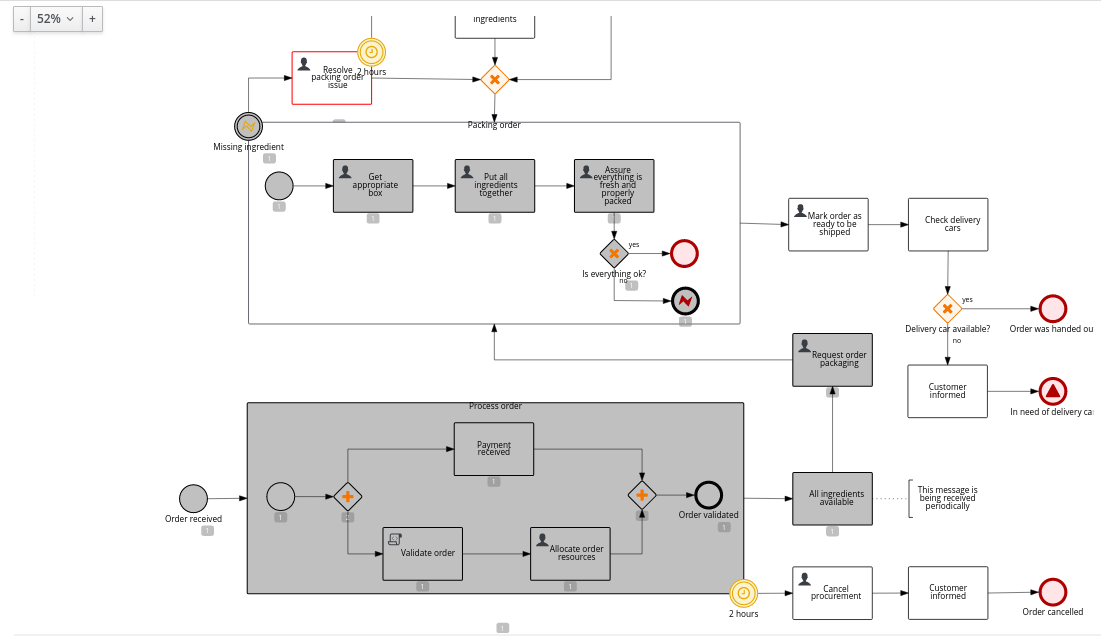
\includegraphics[width=\textwidth]{testing1.png}
    \caption{Process instance diagram of "Order processing" process.}
\end{figure}

\begin{figure}[H]
    \centering
    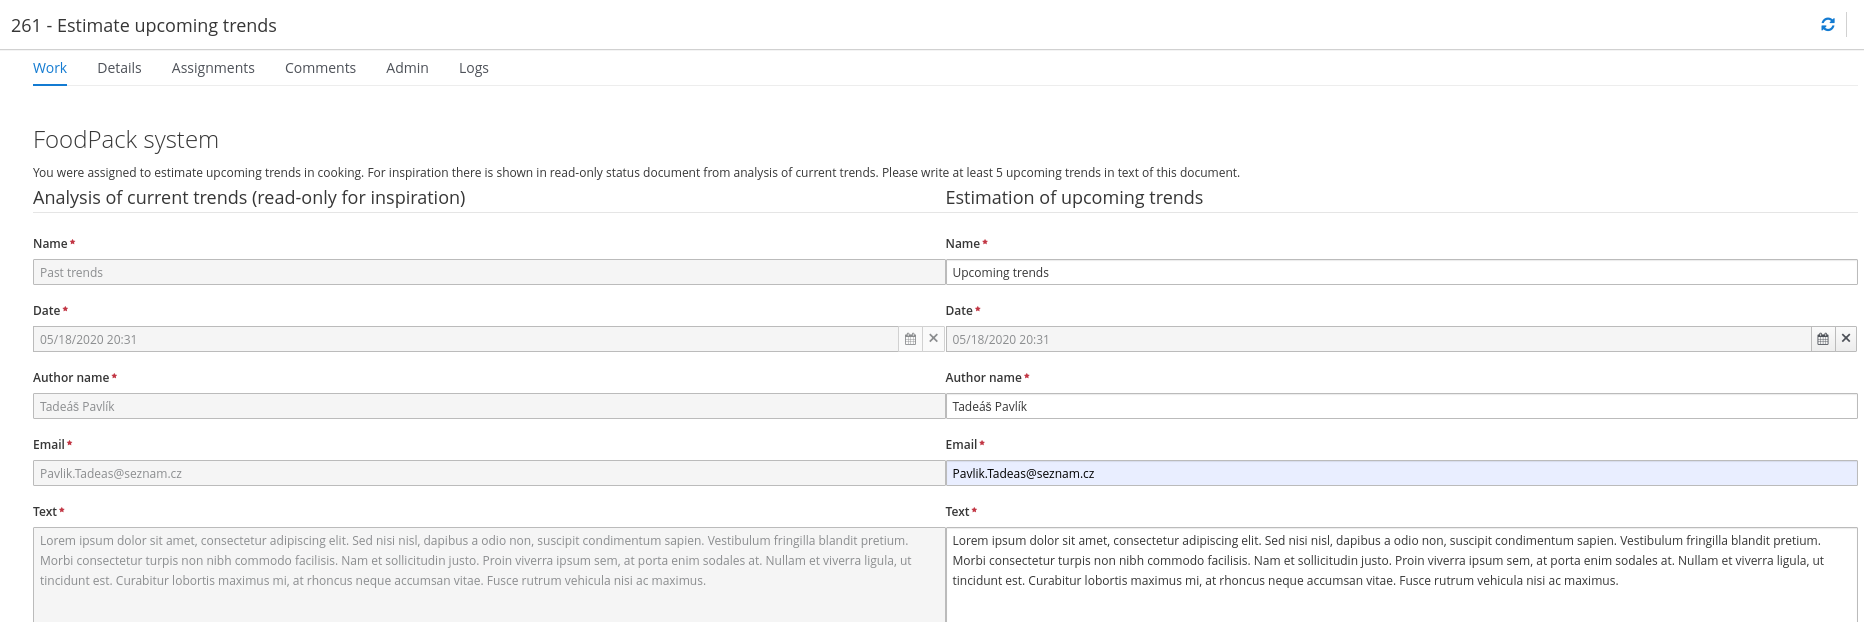
\includegraphics[width=\textwidth]{testing5.png}
    \caption{Form of "Create new recipe" process.}
\end{figure}

\begin{figure}[H]
    \centering
    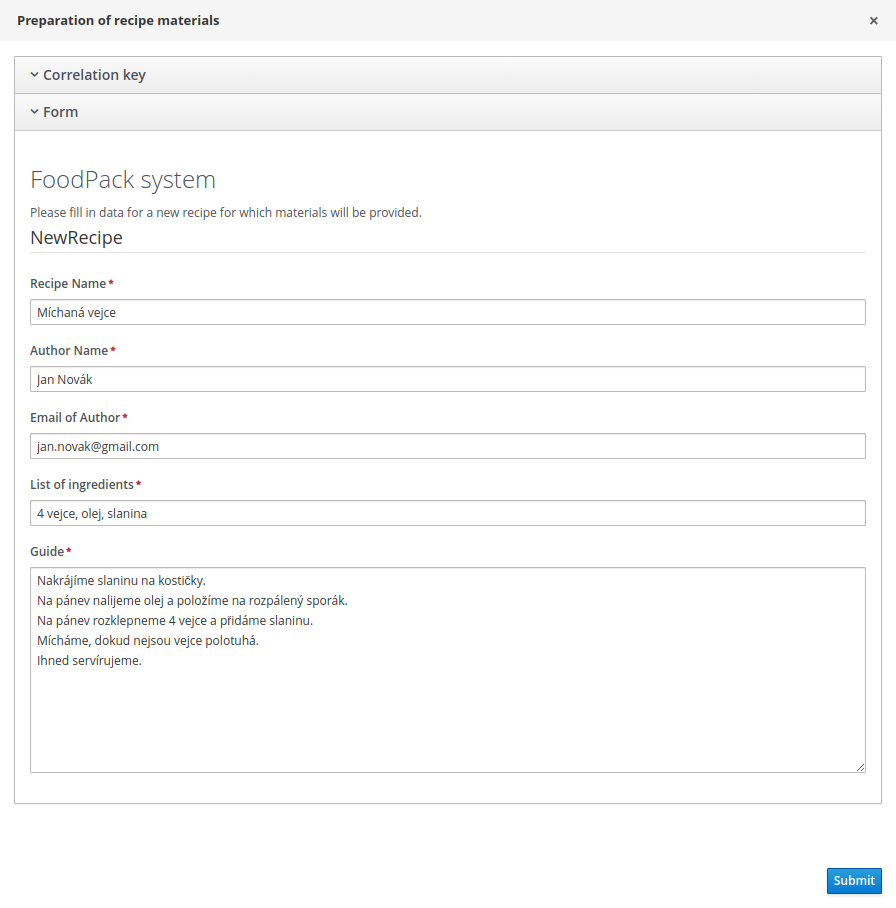
\includegraphics[width=\textwidth]{testing2.png}
    \caption{Form of "Prepare recipe materials" process.}
\end{figure}

\begin{figure}[H]
    \centering
    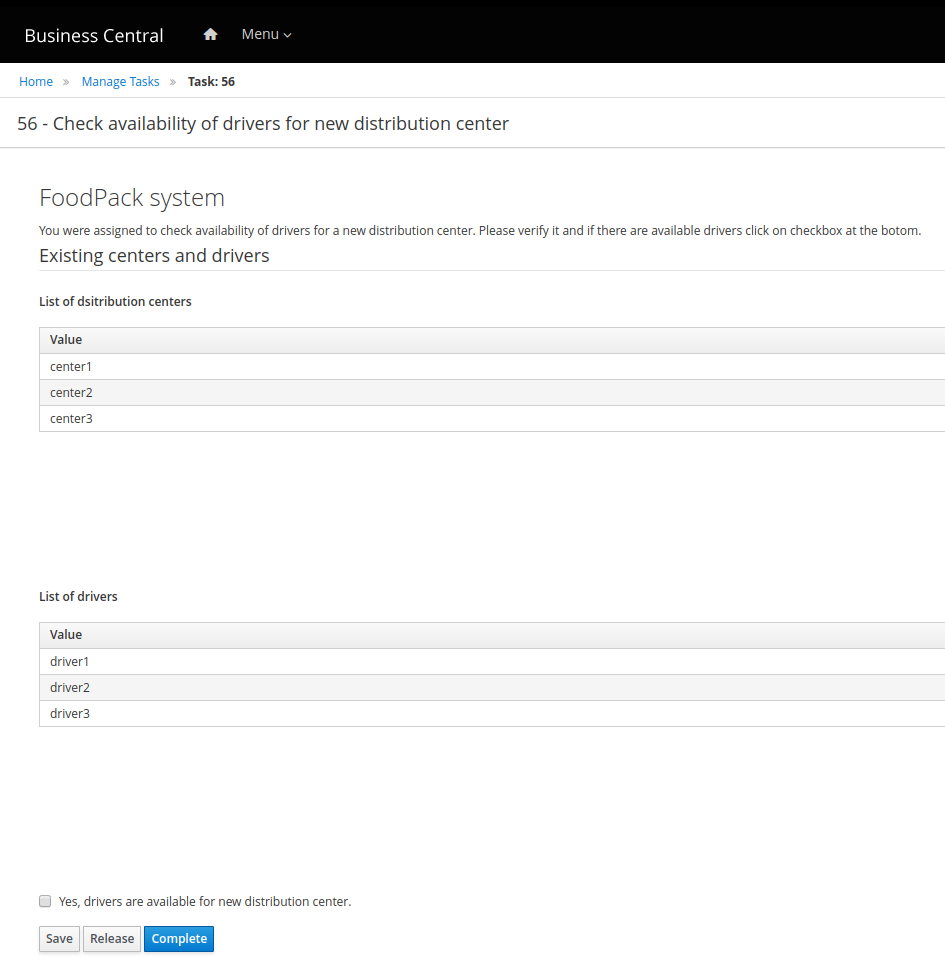
\includegraphics[width=\textwidth]{testing3.png}
    \caption{Form of "Route planning" process.}
\end{figure}

\begin{figure}[H]
    \centering
    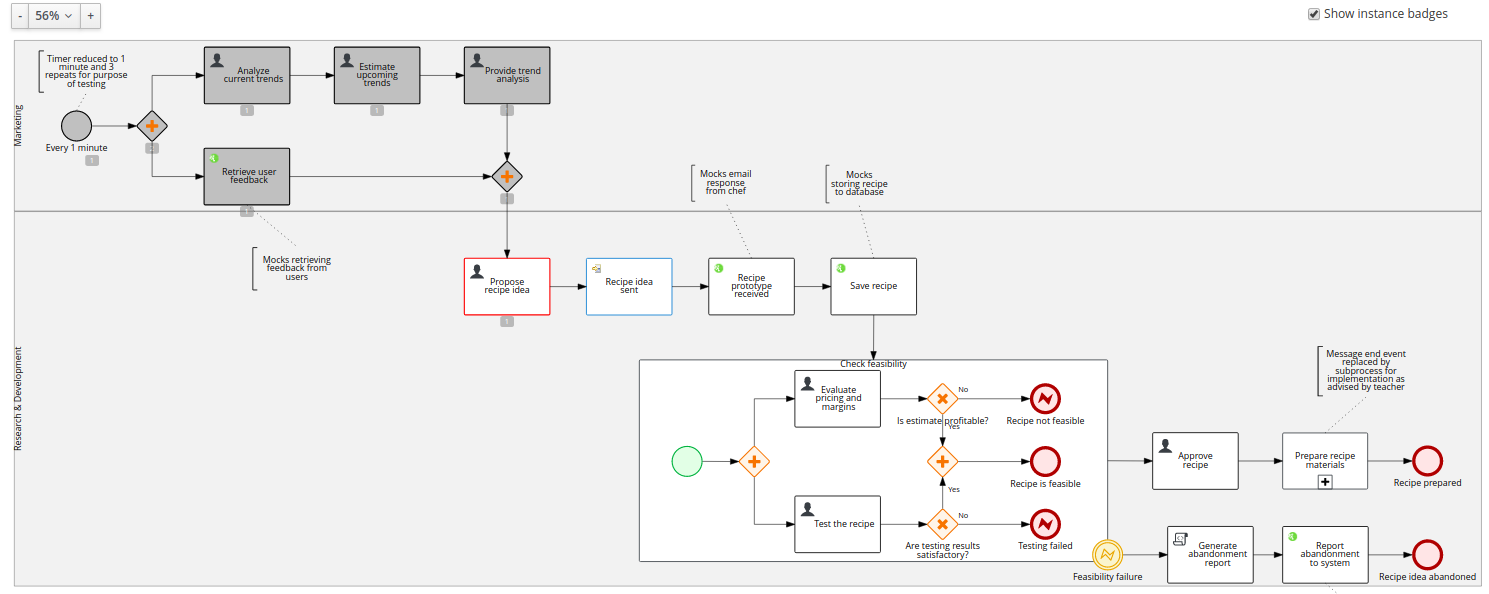
\includegraphics[width=\textwidth]{testing4.png}
    \caption{Process instance diagram of "Create new recipe" process.}
\end{figure}

\newpage

%%%%%%%%%%%%%%%%%%%%%%%%%%%%%%%%%%%%%%%%%%%%%%%%%%%%%%%%%%%%%%%%%%%%%%%%%%%%%%%%%%%%%%%%%%%%%%%%%%%%%%%%%%%%%

\section{Teamwork and tasks}

\subsection{Tadeáš Pavlík (Teamleader)}

\begin{itemize}
    \item Organising the teamwork and managing deadlines
    \item Documentation maintenance
    \item Defined goal, objectives and indicators
    \item Modelled processes in Signavio
    \item Implemented processes
\end{itemize}

\subsection{Jiří Čechák (Business analyst)}

\begin{itemize}
    \item Documentation writing
    \item Defined the mission
    \item Defined goal, objectives and indicators
    \item Modelled processes in Signavio
    \item Tested and debugged implementation of processes
\end{itemize}

\subsection{Tomáš Došlík (Process analyst)}

\begin{itemize}
    \item Documentation writing
    \item Defined the mission
    \item Defined goal, objectives and indicators
    \item Modelled processes in Signavio
    \item Tested and debugged implementation of processes
\end{itemize}

\subsection{Václav Stehlík (BPM/SOA developer)}

\begin{itemize}
    \item Documentation writing
    \item Defined the context
    \item Defined goal, objectives and indicators
    \item Modelled processes in Signavio
    \item Implemented processes
\end{itemize}

\end{document}
